%% \documentclass[12pt,letterpaper]{article}
%% \usepackage[margin=1in,bottom=1in]{geometry} % see geometry.pdf on how to lay out the page. There's lots.
%% 
%% \usepackage{hyperref}
%% \usepackage[journal=jacs]{chemstyle} %Other chemical formatting
%% \usepackage{chemscheme} % Chemical graphics
%% \usepackage{chemcompounds}
%% \usepackage{caption}
%% \usepackage{bpchem} % Chemical compounds
%% \usepackage{setspace}
%% \usepackage{fullpage}
%% \usepackage{graphicx}
%% \usepackage{xspace}
%% \usepackage{booktabs}
%% \usepackage{pdflscape}
%% \usepackage[sort&compress,numbers,super]{natbib}
%% \usepackage{bibentry}
%% %\usepackage{xr}
%% %\externaldocument{isa_ff}
%% \usepackage{amsmath}
%% \usepackage{longtable}
%% \usepackage{xfrac}
%% \usepackage{multirow}
%% \usepackage{dcolumn}
%% \usepackage{siunitx}
%% \usepackage{subcaption}
%% 
%% %eqref
%% \usepackage{letltxmacro}
%% \LetLtxMacro{\originaleqref}{\eqref}
%% \renewcommand{\eqref}{eq.~\originaleqref}
%% \newcommand{\Eqref}{Eq.~\originaleqref}
%% 
%% %figref
%% \newcommand{\figref}[1]{Figure~\ref{#1}}
%% \newcommand{\tabref}[1]{Table~\ref{#1}}
%% \newcommand{\secref}[1]{Section~\ref{#1}}
%% 
%% \newcommand{\super}[1]{\textsuperscript{#1}}
%% \newcommand{\sub}[1]{\textsubscript{#1}}
%% \renewcommand{\thefootnote}{\fnsymbol{footnote}}
%% \newcommand{\ra}[1]{\renewcommand{\arraystretch{#1}}}
%% \newcommand{\centercell}[1]{\multicolumn{1}{C}{#1}}
%% 
%% % Supplementary Information Labels
%% \newcommand{\beginsupplement}{%
%%         \setcounter{table}{0}
%%         \renewcommand{\thetable}{S\arabic{table}}%
%%         \setcounter{figure}{0}
%%         \renewcommand{\thefigure}{S\arabic{figure}}%
%%         \setcounter{section}{0}
%%         \renewcommand{\thesection}{S\arabic{section}}%
%%      }
%% 
%% \newcommand{\citeboth}[1]{\citeauthor{#1}\cite{#1}\xspace}
%% \newcommand*{\citen}[1]{%
%%   \begingroup
%%     \romannumeral-`\x % remove space at the beginning of \setcitestyle
%%     \setcitestyle{numbers}%
%%     ref. \cite{#1}%
%%   \endgroup   
%% }
%% 
%% \hyphenation{homodimer}
%% 
%% 
%% % ISA-FF Paper lingo
%% 
%% \newcommand{\co}{\BPChem{CO\_2}\xspace}
%% \newcommand{\ho}{\BPChem{H\_2O}\xspace}
%% \newcommand{\nh}{\BPChem{NH\_3}\xspace}
%% \newcommand{\cl}{\BPChem{CH\_3Cl}\xspace}
%% 
%% 
%% \newcommand{\isa}{BS-ISA\xspace}
%% \newcommand{\isoff}{Iso-Iso FF\xspace}
%% \newcommand{\isaff}{Aniso-Aniso FF\xspace}
%% \newcommand{\mastiff}{MASTIFF\xspace}
%% \newcommand{\saptff}{Born-Mayer-IP FF\xspace}
%% \newcommand{\bmsisaff}{Born-Mayer-sISA FF\xspace}
%% \newcommand{\ljff}{LJ FF\xspace}
%% \newcommand{\sapt}{DFT-SAPT (PBE0/AC)\xspace}
%% \newcommand{\avtz}{aug-cc-pVTZ\xspace}
%% \newcommand{\A}{\ensuremath{A_{ij}}\xspace}
%% \newcommand{\B}{\ensuremath{B_{ij}}\xspace}
%% \newcommand{\C}{\ensuremath{C_{ij,n}}\xspace}
%% \newcommand{\R}{\ensuremath{r_{ij}}\xspace}
%% 
%% \newcommand{\dhf}{\ensuremath{\delta^{\text{HF}}}\xspace}
%% 
%% \newcommand{\Asr}[1]{\ensuremath{A^{\text{sr}}_{#1}}\xspace}
%% \newcommand{\Aex}[1]{\ensuremath{A^{\text{exch}}_{#1}}\xspace}
%% \newcommand{\Ael}[1]{\ensuremath{A^{\text{elst}}_{#1}}\xspace}
%% \newcommand{\Apen}[1]{\ensuremath{A^{\text{pen}}_{#1}}\xspace}
%% \newcommand{\Aind}[1]{\ensuremath{A^{\text{ind}}_{#1}}\xspace} % AJM Not ind,sr !!!
%% \newcommand{\Adhf}[1]{\ensuremath{A^{\dhf}_{#1}}\xspace} % AJM Not ind,sr !!!
%% 
%% \newcommand{\Bisa}[1]{\ensuremath{B^{\text{ISA}}_{#1}}\xspace}
%% \newcommand{\Bip}[1]{\ensuremath{B^{\text{IP}}_{#1}}\xspace}
%% 
%% \newcommand{\etot}{\ensuremath{E_{\text{int}}}\xspace}
%% \newcommand{\erep}{\ensuremath{E^{\text{exch}}}\xspace}
%% \newcommand{\eelst}{\ensuremath{E^{\text{elst}}}\xspace}
%% \newcommand{\eind}{\ensuremath{E^{\text{ind}}}\xspace}
%% \newcommand{\edhf}{\ensuremath{E^{\dhf}}\xspace}
%% \newcommand{\edisp}{\ensuremath{E^{\text{disp}}}\xspace}
%% 
%% \newcommand{\vtot}{\ensuremath{V_{\text{FF}}}\xspace}
%% \newcommand{\vrep}{\ensuremath{V^{\text{exch}}}\xspace}
%% \newcommand{\vcp}{\ensuremath{V^{\text{pen}}}\xspace}
%% \newcommand{\vsrind}{\ensuremath{V^{\text{ind,sr}}}\xspace}
%% \newcommand{\vsrdisp}{\ensuremath{V^{\text{disp,sr}}}\xspace}
%% \newcommand{\velst}{\ensuremath{V^{\text{elst}}}\xspace}
%% \newcommand{\vind}{\ensuremath{V^{\text{ind}}}\xspace}
%% \newcommand{\vdhf}{\ensuremath{V^{\dhf}}\xspace}
%% \newcommand{\vdisp}{\ensuremath{V^{\text{disp}}}\xspace}
%% \newcommand{\vlr}{\ensuremath{V_{lr}}\xspace}
%% \newcommand{\vmultipole}{\ensuremath{\sum\limits_{tu}Q_t^iT_{tu}Q_u^j}\xspace}
%% \newcommand{\vdrude}{\ensuremath{V_{\text{shell}}}\xspace}
%% \newcommand{\vdrudeind}{\ensuremath{V_{\text{shell}}^{(2)}}\xspace}
%% \newcommand{\vdrudescf}{\ensuremath{V_{\text{shell}}^{(3-\infty)}}\xspace}
%% 
%% \newcommand{\mse}{\ensuremath{\lVert\text{MSE}\rVert}\xspace}
%% 
%% \title{\textbf{Supporting Information} \\ for \\
%% `New angles on standard force fields: a general approach for incorporating
%% atomic-level anisotropy'
%% }
%% \author{Mary J. Van Vleet, Alston J. Misquitta, J.R. Schmidt}
%% %\date{April 23, 2015} % delete this line to display the current date
%% 
%% \begin{document}
%% \beginsupplement
%% \maketitle
%% \tableofcontents
%% 
%% 
%% %%%%%%%%%%%%%%%%%%%%%%%%%%%%%%%%% SI %%%%%%%%%%%%%%%%%%%%%%%%%%%%%%%%%%%%%%%%%%%%%%
%% \onehalfspacing
%% 
%% \begin{section}{\mse Values}
%% 
%%     %%%%%%%%%%%% Average MSE %%%%%%%%%%%%%%%
%%     \begin{figure}
%%     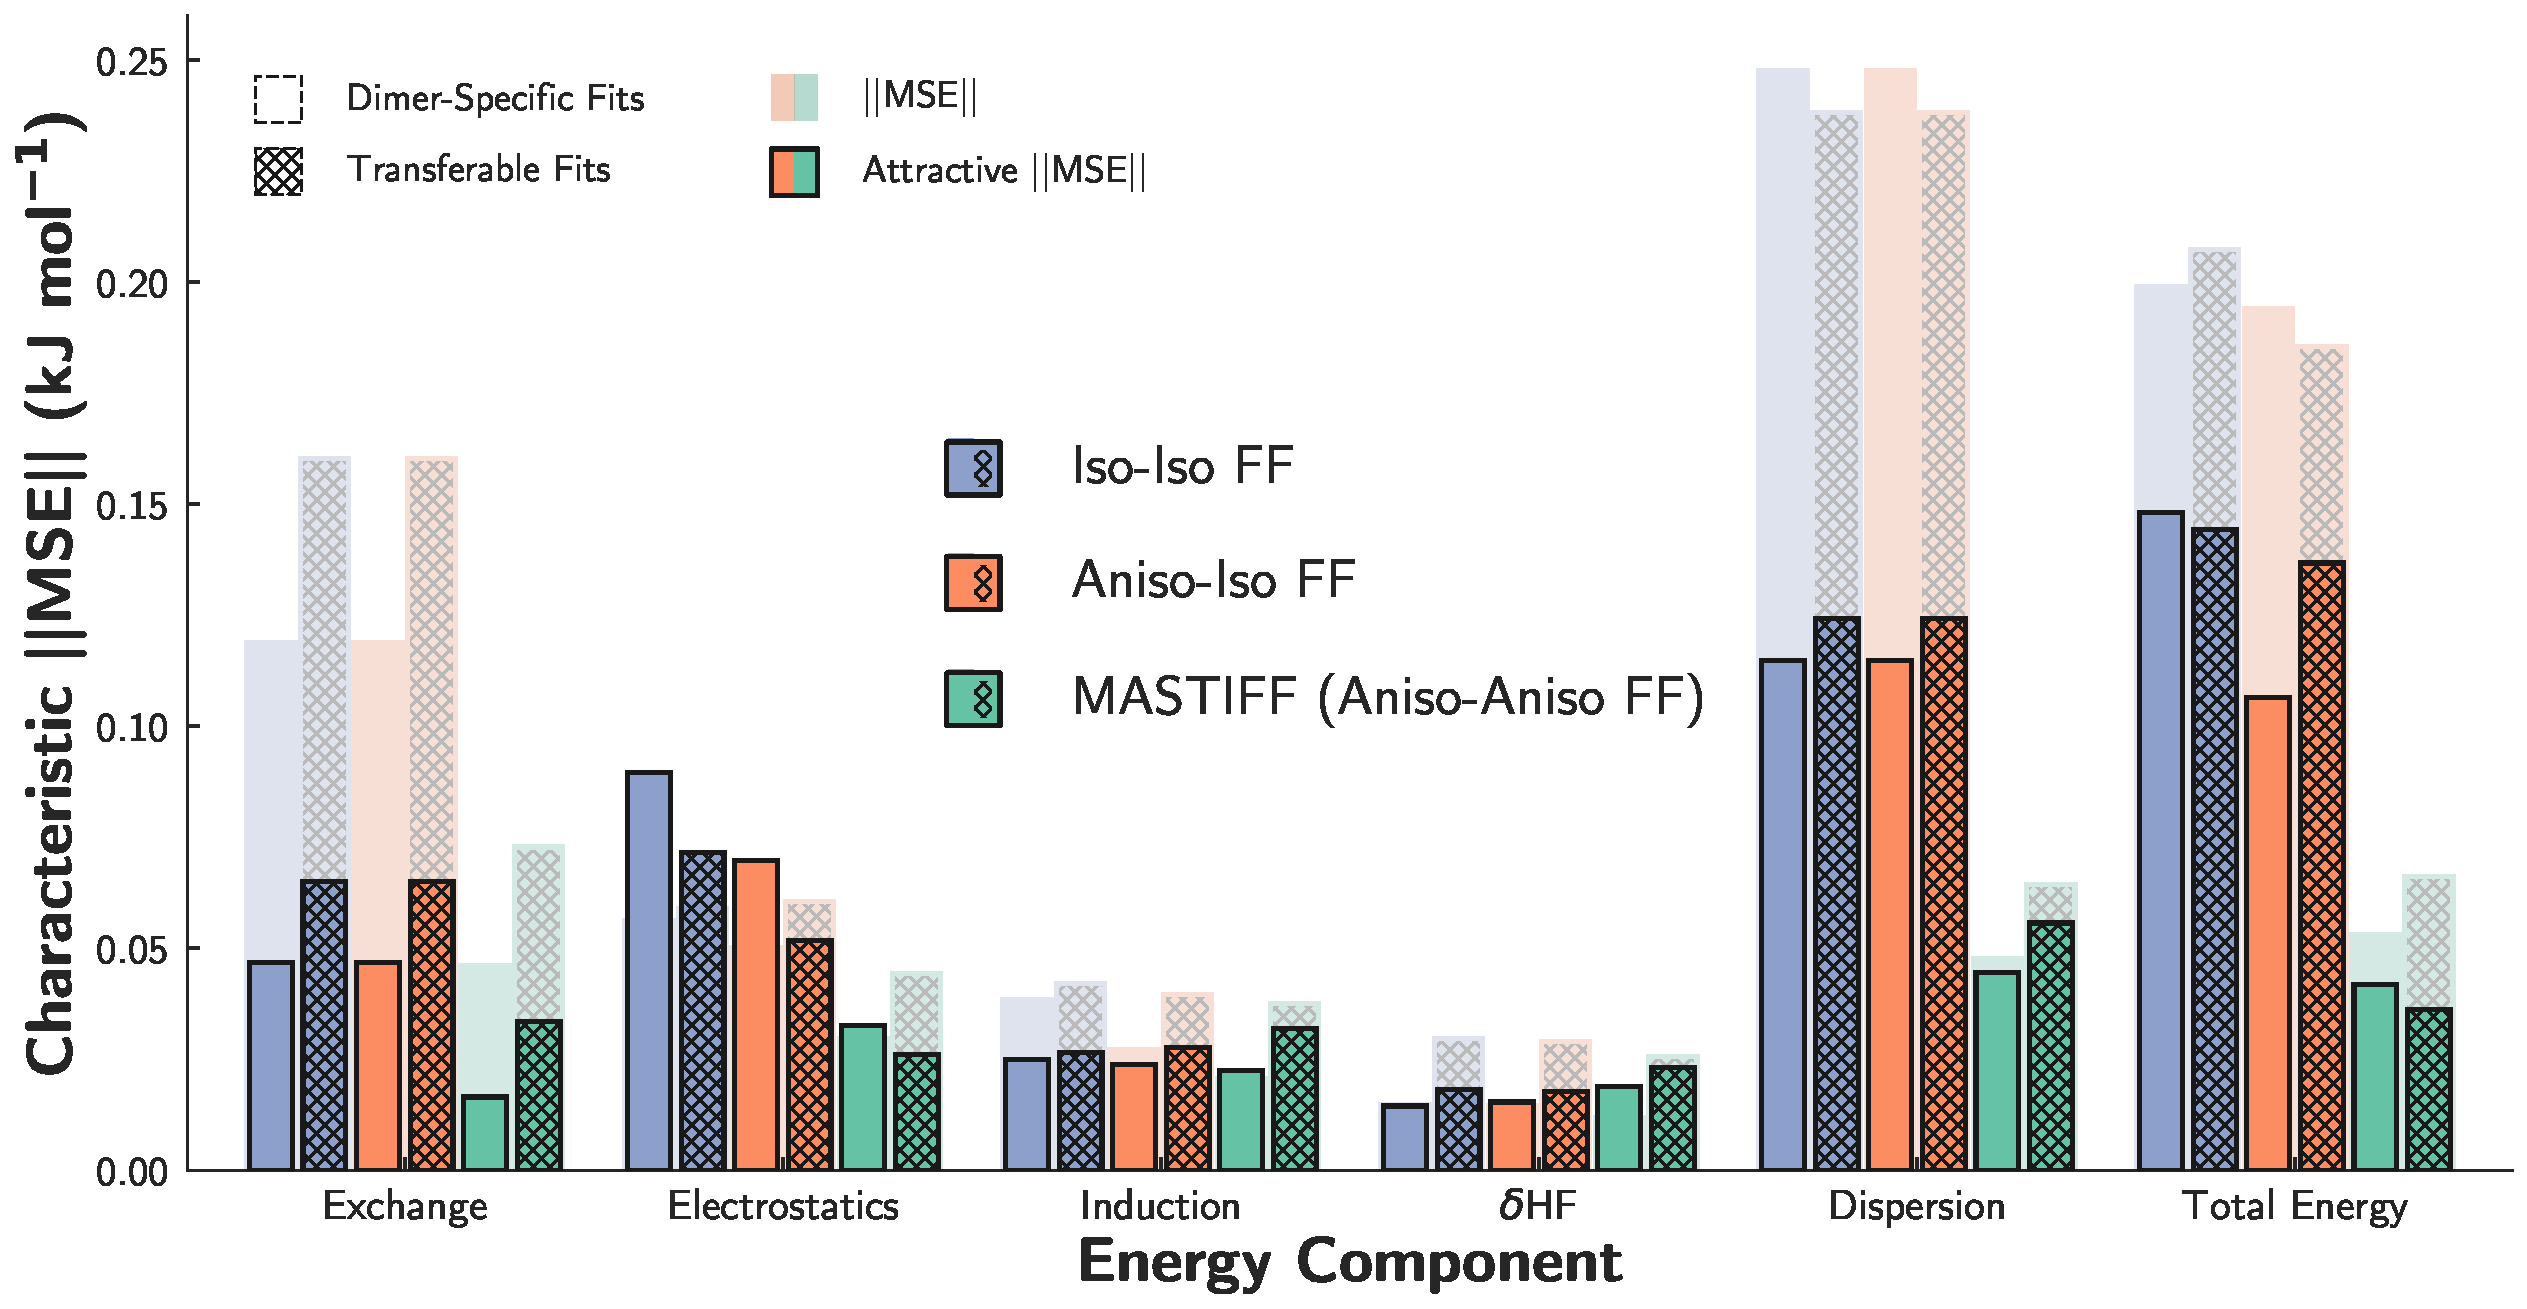
\includegraphics[width=0.9\textwidth]{../rmse_comparisons/transferability_mae_errors.pdf}
%%     \caption{
%%     Characteristic \mse (as described in the main text) for the \isoff
%% (purple), \isaff (orange), and \mastiff (green) over the 91
%%     dimer test set. Terms and labels are as in the main text.
%%             }
%%     \label{fig:mse}
%%     \end{figure}
%%     %%%%%%%%%%%% Average MSE %%%%%%%%%%%%%%%
%% 
%% \end{section}
%% \clearpage
%% 
%% 
%% \begin{section}{Improvement Ratios}
%% 
%%     %%%%%%%%%%%% Average MSE %%%%%%%%%%%%%%%
%%     \begin{table}
%%     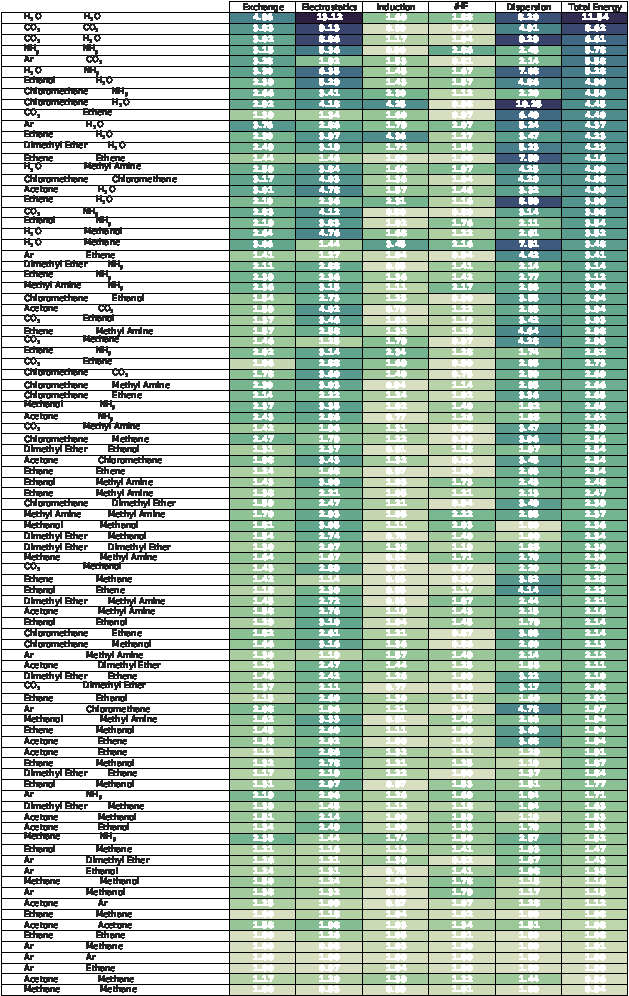
\includegraphics[width=0.8\textwidth]{all_error_ratios.pdf}
%%     \caption{
%% Improvement ratios (see main text) for all species in the 91 dimer test set.
%%             }
%%     \label{tab:all_ratios}
%%     \end{table}
%%     %%%%%%%%%%%% Average MSE %%%%%%%%%%%%%%%
%% 
%% \end{section}
%% \clearpage
%% 
%% 
%% 
%% \begin{section}{Monomer Geometries}
%% \label{sec:geometries}
%% 
%% Geometries for each molecule in the 91 dimer test set are listed below, in
%% alphabetical order. Also listed are the relevant energies (highest occupied
%% molecular orbital and ionization potential) for the asymptotic correction
%% required in DFT-SAPT calculations of each molecule. All asymptotic corrections
%% were performed at a PBE0/\avtz level of theory. Distances and energies are in
%% a.u.
%% 
%% \scriptsize
%% \centering
\renewcommand\arraystretch{1.1}
\newcolumntype{L}{D{.}{.}{2,6}}
\begin{longtable}{@{}rLLL@{}}
\caption{Cartesian coordinates for each molecule in the 91 dimer test set. HOMO
and I.P. values, necessary for DFT-SAPT calculations, are also shown. All units
are in a.u.}
\label{tab:geometries}
\\

\endfirsthead

\multicolumn{4}{c}%
{{\bfseries \tablename\ \thetable{} -- continued from previous page}} \\
\hline
\endhead
%% \toprule
%% Atomtype & 
%% \multicolumn{1}{c}{$Q_{00 }$} &
%% \multicolumn{1}{c}{$Q_{10 }$} &
%% \multicolumn{1}{c}{$Q_{11c}$} &
%% \multicolumn{1}{c}{$Q_{11s}$} &
%% \multicolumn{1}{c}{$Q_{20 }$} &
%% \multicolumn{1}{c}{$Q_{21c}$} &
%% \multicolumn{1}{c}{$Q_{21s}$} &
%% \multicolumn{1}{c}{$Q_{22c}$} &
%% \multicolumn{1}{c}{$Q_{22s}$} \\
%% \midrule
%% \endhead
%% 
%% \bottomrule
%% \endfoot

\multicolumn{4}{l}{\textbf{Acetone}}  \\*
\toprule
C      &   0.000000  &   0.000000  &  -2.280333 \\* 
O      &   0.000000  &   0.000000  &   0.000000 \\* 
C      &   0.000000  &   2.435101  &  -3.793814 \\* 
C      &   0.000000  &  -2.435101  &  -3.793814 \\* 
H      &   0.000000  &   4.050439  &  -2.525430 \\* 
H      &   0.000000  &  -4.050439  &  -2.525430 \\* 
H      &   1.657668  &   2.514281  &  -5.019869 \\* 
H      &  -1.657668  &   2.514281  &  -5.019869 \\* 
H      &  -1.657668  &  -2.514281  &  -5.019869 \\* 
H      &   1.657668  &  -2.514281  &  -5.019869 \\* 

\bottomrule
\multicolumn{2}{l}{HOMO:} &
-0.266741       
\\*
\multicolumn{2}{l}{I.P.:} &
0.35386979
\\*
\\

\multicolumn{4}{l}{\textbf{Ar}}  \\*
\toprule
Ar     &   0.000000  &   0.000000  &   0.000000 \\* 

\bottomrule
\multicolumn{2}{l}{HOMO:} &
-0.440599       
\\*
\multicolumn{2}{l}{I.P.:} &
0.58049447
\\*
\\

\multicolumn{4}{l}{\textbf{Chloromethane}}  \\*
\toprule
C      &   0.000000  &   0.000000  &  -3.365602 \\* 
Cl     &   0.000000  &   0.000000  &   0.000000 \\* 
H      &   1.969851  &   0.000000  &  -4.102784 \\* 
H      &  -0.984925  &   1.705856  &  -4.102784 \\* 
H      &  -0.984925  &  -1.705856  &  -4.102784 \\* 

\bottomrule
\multicolumn{2}{l}{HOMO:} &
-0.313074       
\\*
\multicolumn{2}{l}{I.P.:} &
0.41507894
\\*
\\

\multicolumn{4}{l}{\textbf{CO\sub2}}  \\*
\toprule
C      &   0.000000  &   0.000000  &   0.000000 \\* 
O      &   0.000000  &   0.000000  &   2.196051 \\* 
O      &   0.000000  &   0.000000  &  -2.196051 \\* 

\bottomrule
\multicolumn{2}{l}{HOMO:} &
-0.394037       
\\*
\multicolumn{2}{l}{I.P.:} &
0.51235857
\\*
\\

\multicolumn{4}{l}{\textbf{Dimethyl Ether}}  \\*
\toprule
O      &   0.000000  &   0.000000  &   0.000000 \\* 
C      &   0.000000  &   2.205121  &  -1.495718 \\* 
C      &   0.000000  &  -2.205121  &  -1.495718 \\* 
H      &   0.000000  &   3.871860  &  -0.266451 \\* 
H      &   0.000000  &  -3.871860  &  -0.266451 \\* 
H      &   1.691305  &   2.227420  &  -2.690781 \\* 
H      &  -1.691305  &   2.227420  &  -2.690781 \\* 
H      &  -1.691305  &  -2.227420  &  -2.690781 \\* 
H      &   1.691305  &  -2.227420  &  -2.690781 \\* 

\bottomrule
\multicolumn{2}{l}{HOMO:} &
-0.272835       
\\*
\multicolumn{2}{l}{I.P.:} &
0.36469012
\\*
\\

\multicolumn{4}{l}{\textbf{Ethane}}  \\*
\toprule
C      &   0.000000  &   0.000000  &   0.000000 \\* 
C      &   0.000000  &   0.000000  &  -2.902619 \\* 
H      &  -1.926009  &   0.000000  &   0.735670 \\* 
H      &   0.963004  &   1.667872  &   0.735670 \\* 
H      &   0.963004  &  -1.667872  &   0.735670 \\* 
H      &   1.926009  &   0.000000  &  -3.638290 \\* 
H      &  -0.963004  &  -1.667872  &  -3.638290 \\* 
H      &  -0.963004  &   1.667872  &  -3.638290 \\* 

\bottomrule
\multicolumn{2}{l}{HOMO:} &
-0.353672       
\\*
\multicolumn{2}{l}{I.P.:} &
0.45125450
\\*
\\

\multicolumn{4}{l}{\textbf{Ethanol}}  \\*
\toprule
C      &   4.487344  &  -0.256436  &   0.000000 \\* 
C      &   2.242538  &   1.511403  &   0.000000 \\* 
O      &   0.000000  &   0.000000  &   0.000000 \\* 
H      &  -1.392728  &   1.194685  &   0.000000 \\* 
H      &   6.208128  &   0.902911  &   0.000000 \\* 
H      &   4.356008  &  -1.440160  &   1.675998 \\* 
H      &   4.356008  &  -1.440160  &  -1.675998 \\* 
H      &   2.199641  &   2.699285  &   1.672786 \\* 
H      &   2.199641  &   2.699285  &  -1.672786 \\* 

\bottomrule
\multicolumn{2}{l}{HOMO:} &
-0.287342       
\\*
\multicolumn{2}{l}{I.P.:} &
0.38582676
\\*
\\

\multicolumn{4}{l}{\textbf{Ethene}}  \\*
\toprule
C      &   0.000000  &   0.000000  &   0.000000 \\* 
C      &   0.000000  &   0.000000  &  -2.530343 \\* 
H      &   0.000000  &   1.755367  &   1.063160 \\* 
H      &   0.000000  &  -1.755367  &   1.063160 \\* 
H      &   0.000000  &   1.755367  &  -3.593503 \\* 
H      &   0.000000  &  -1.755367  &  -3.593503 \\* 

\bottomrule
\multicolumn{2}{l}{HOMO:} &
-0.288580       
\\*
\multicolumn{2}{l}{I.P.:} &
0.38518748
\\*
\\

\multicolumn{4}{l}{\textbf{H\sub2O}}  \\*
\toprule
O      &   0.000000  &   0.000000  &   0.000000 \\* 
H      &   0.000000  &   1.430901  &  -1.108324 \\* 
H      &   0.000000  &  -1.430901  &  -1.108324 \\* 

\bottomrule
\multicolumn{2}{l}{HOMO:} &
-0.333820       
\\*
\multicolumn{2}{l}{I.P.:} &
0.46592291
\\*
\\

\multicolumn{4}{l}{\textbf{Methane}}  \\*
\toprule
C      &   0.000000  &   0.000000  &   0.000000 \\* 
H      &   1.185992  &   1.185992  &   1.185992 \\* 
H      &   1.185992  &  -1.185992  &  -1.185992 \\* 
H      &  -1.185992  &   1.185992  &  -1.185992 \\* 
H      &  -1.185992  &  -1.185992  &   1.185992 \\* 

\bottomrule
\multicolumn{2}{l}{HOMO:} &
-0.403996       
\\*
\multicolumn{2}{l}{I.P.:} &
0.51955025
\\*
\\

\multicolumn{4}{l}{\textbf{Methanol}}  \\*
\toprule
C      &   0.000000  &   2.696639  &   0.000000 \\* 
O      &   0.000000  &   0.000000  &   0.000000 \\* 
H      &  -1.947174  &   3.401885  &   0.000000 \\* 
H      &   0.973776  &   3.401885  &   1.686392 \\* 
H      &   0.973776  &   3.401885  &  -1.686392 \\* 
H      &   1.709635  &  -0.584303  &   0.000000 \\* 

\bottomrule
\multicolumn{2}{l}{HOMO:} &
-0.292049       
\\*
\multicolumn{2}{l}{I.P.:} &
0.39901686
\\*
\\

\multicolumn{4}{l}{\textbf{Methyl Amine}}  \\*
\toprule
C      &   0.000000  &   2.779976  &   0.000000 \\* 
N      &   0.000000  &   0.000000  &   0.000000 \\* 
H      &  -1.887836  &   3.667203  &   0.000000 \\* 
H      &   1.026877  &   3.452719  &   1.668817 \\* 
H      &   1.026877  &   3.452719  &  -1.668817 \\* 
H      &  -0.960170  &  -0.632113  &  -1.537670 \\* 
H      &  -0.960170  &  -0.632113  &   1.537670 \\* 

\bottomrule
\multicolumn{2}{l}{HOMO:} &
-0.255840       
\\*
\multicolumn{2}{l}{I.P.:} &
0.35552078
\\*
\\

\multicolumn{4}{l}{\textbf{NH\sub3}}  \\*
\toprule
N      &   0.000000  &   0.000000  &   0.000000 \\* 
H      &   0.000000  &  -1.771996  &  -0.721119 \\* 
H      &   1.534647  &   0.886093  &  -0.721119 \\* 
H      &  -1.534647  &   0.886093  &  -0.721119 \\* 

\bottomrule
\multicolumn{2}{l}{HOMO:} &
-0.284421       
\\*
\multicolumn{2}{l}{I.P.:} &
0.39987353
\\*
\\


\end{longtable}



%% \normalsize
%% 
%% 
%% \end{section}
\begin{section}{Local Axis Definitions}
\label{sec:mastiff-local_axis_defs}

For each molecule in the 91 dimer test set, listed below are any atom types
which have been treated anisotropically. For each anisotropic atom type, the
approximate symmetry and all
terms included in the spherical harmonic expansion are listed to the right of
the atom type. Additionally, the local axis reference frame for each
anisotropic atom type is
defined in the Axes subsection using the z-then-x convention employed by
AMOEBA and other potentials. The first column
of the axes subsection denotes the index of the anisotropic atom (atom
ordering as in \cref{sec:appendices-monomers}), and the second column denotes whether the
z or x axis is being defined. For certain local symmetries, the
choice of x-axis is unimportant, and so not every anisotropic atom type has a
defined x-axis. 
The remaining columns define the direction vector for the
axis in terms of atomic indices. The first index (often
the anisotropic atom itself) lists the start of the vector, and the endpoint
of the vector is defined as the midpoint of all subsequently listed atoms.

To use water as an example, the oxygen atom is treated anisotropically
using a spherical harmonic expansion that includes y10, y20, and y22c terms
(notation as in \citen{stone2013theory}). The z-axis points from the oxygen to
the midpoint between the two hydrogens, and the xz plane (and subsequently the
x-axis) is defined by one of
the O--H bonds. 

\begin{subsection}{Acetone}
\begin{verbatim}
OC  c2v     y10 y20 y22c

Axes
ATOM#   AXIS (z or x)   Atomic Indices defining vector (either 2 or more
integers)
1 z 1 0
1 x 0 2
\end{verbatim}
\end{subsection}
\begin{subsection}{Ar}
\begin{verbatim}
Ar

Axes
ATOM#   AXIS (z or x)   Atomic Indices defining vector (either 2 or more
integers)
\end{verbatim}
\end{subsection}
\begin{subsection}{Chloromethane}
\begin{verbatim}
Chloromethane
Cl c3v     y10 y20

Axes
ATOM#   AXIS (z or x)   Atomic Indices defining vector (either 2 or more
integers)
1 z 1 0
\end{verbatim}
\end{subsection}
\begin{subsection}{Carbon Dioxide}
\begin{verbatim}
CO2
OCO cinfv y10 y20
CCO2 dinfh y20

Axes
ATOM#   AXIS (z or x)   Atomic Indices defining vector (either 2 or more
integers)
0 z 0 1
1 z 1 0
2 z 2 0
\end{verbatim}
\end{subsection}
\begin{subsection}{Dimethyl Ether}
\begin{verbatim}
Dimethyl Ether
O c2v y10 y20 y22c

Axes
ATOM#   AXIS (z or x)   Atomic Indices defining vector (either 2 or more
integers)
0 z 0 1 2
0 x 0 1
\end{verbatim}
\end{subsection}
\begin{subsection}{Ethane}
\begin{verbatim}
Ethane

Axes
ATOM#   AXIS (z or x)   Atomic Indices defining vector (either 2 or more
integers)
\end{verbatim}
\end{subsection}
\begin{subsection}{Ethanol}
\begin{verbatim}
Ethanol
OH c2v y10 y20 y22c
HO cinfv y10 y20

Axes
ATOM#   AXIS (z or x)   Atomic Indices defining vector (either 2 or more
integers)
2 z 2 1 3
2 x 2 1
3 z 3 2
\end{verbatim}
\end{subsection}
\begin{subsection}{Ethene}
\begin{verbatim}
Ethene
CM c2v y22c
HM cinfv y10 y20

Axes
ATOM#   AXIS (z or x)   Atomic Indices defining vector (either 2 or more
integers)
0 z 0 1
0 x 0 2
1 z 1 0
1 x 1 4
2 z 2 0
3 z 3 0
4 z 4 1
5 z 5 1
\end{verbatim}
\end{subsection}
\begin{subsection}{Water}
\begin{verbatim}
H2O
OH2 c2v y10 y20 y22c
H2O cinfv y10 y20

Axes
ATOM#   AXIS (z or x)   Atomic Indices defining vector (either 2 or more
integers)
0 z 0 1 2
0 x 0 1
1 z 1 0
2 z 2 0
\end{verbatim}
\end{subsection}
\begin{subsection}{Methane}
\begin{verbatim}
Methane

Axes
ATOM#   AXIS (z or x)   Atomic Indices defining vector (either 2 or more
integers)
\end{verbatim}
\end{subsection}
\begin{subsection}{Methanol}
\begin{verbatim}
Methanol
OH1 c2v y10 y20 y22c
HO1 cinfv y10 y20

Axes
ATOM#   AXIS (z or x)   Atomic Indices defining vector (either 2 or more
integers)
1 z 1 0 5
1 x 1 0
5 z 5 1
\end{verbatim}
\end{subsection}
\begin{subsection}{Methyl Amine}
\begin{verbatim}
Methyl Amine
N1 c2v y10 y20 y22c
HN1 cinfv y10 y20

Axes
ATOM#   AXIS (z or x)   Atomic Indices defining vector (either 2 or more
integers)
1 z 1 0 5 6
1 x 1 0
5 z 5 1
6 z 6 1
\end{verbatim}
\end{subsection}
\begin{subsection}{Ammonia}
\begin{verbatim}
Ammonia
N c3v y10 y20
HN cinfv y10 y20

Axes
ATOM#   AXIS (z or x)   Atomic Indices defining vector (either 2 or more
integers)
0 z 0 1 2 3
0 x 0 1
1 z 1 0
2 z 2 0
3 z 3 0

\end{verbatim}
\end{subsection}


\end{section}
%% \clearpage
%% \begin{section}{\mastiff Parameters and Fits}
%% %\label{sec:mastiff-fits}
%% 
%% 
%% \mastiff parameters for each homomonomeric dimer are given
%% in the attached homodimer\_params.tgz file. Parameters for \isoff
%% and/or \isaff can be made available upon request. For each dimer, multipole
%% moments are listed in a .mom file, polarization parameters (thole damping
%% parameters, spring constants, and drude charges) are found in the .param file, and all other
%% parameters can be found in the fit\_exp\_coeffs\_unconstrained.out file. With the
%% exception of anisotropy parameters, which are unitless, all parameters are in
%% atomic units. 
%% 
%% homodimer\_params.tgz additionally contains fitting results for each
%% homomonomeric species. Fitting results for \isaff and for heteromonomeric
%% species can be made available upon request. For each dimer, geometries and
%% DFT-SAPT results are given in the .sapt file, and both SAPT and \mastiff
%% energies are listed (respectively, and in the same order as the .sapt file) for each energy
%% component (as discussed in the main text) in a corresponding .dat file. 
%% The energies in these .dat files correspond to the scatterplots shown in
%% \secref{sec:homodimer_fits}. Once again, all quantities are in atomic units,
%% with the exception that the energies in the .sapt file are in mH.
%% 
%% \end{section}
%% \begin{section}{\mastiff-CC Parameters}
%% 
%% \mastiff-CC paramters for \co, \nh, \cl, and \ho are given (in a .xml format
%% which can be read directly into OpenMM) in the attached
%% mastiff-cc\_reference.tgz file. Aside from the \co force field, many-body
%% effects have not been included/tested for the other \mastiff-CC force fields, and so
%% caution is advised before using these potentials in bulk simulations. Any use of
%% the \mastiff-CC potentials should reference this work and \citen{VanVleet2016}.
%% 
%% \end{section}
\begin{section}{Homodimer Fits}
\label{sec:mastiff-fits}

    %%%%%%%% All Scatter %%%%%%%%%%
    \begin{figure}
    \begin{subfigure}{\textwidth}
        \caption{Acetone Dimer}
        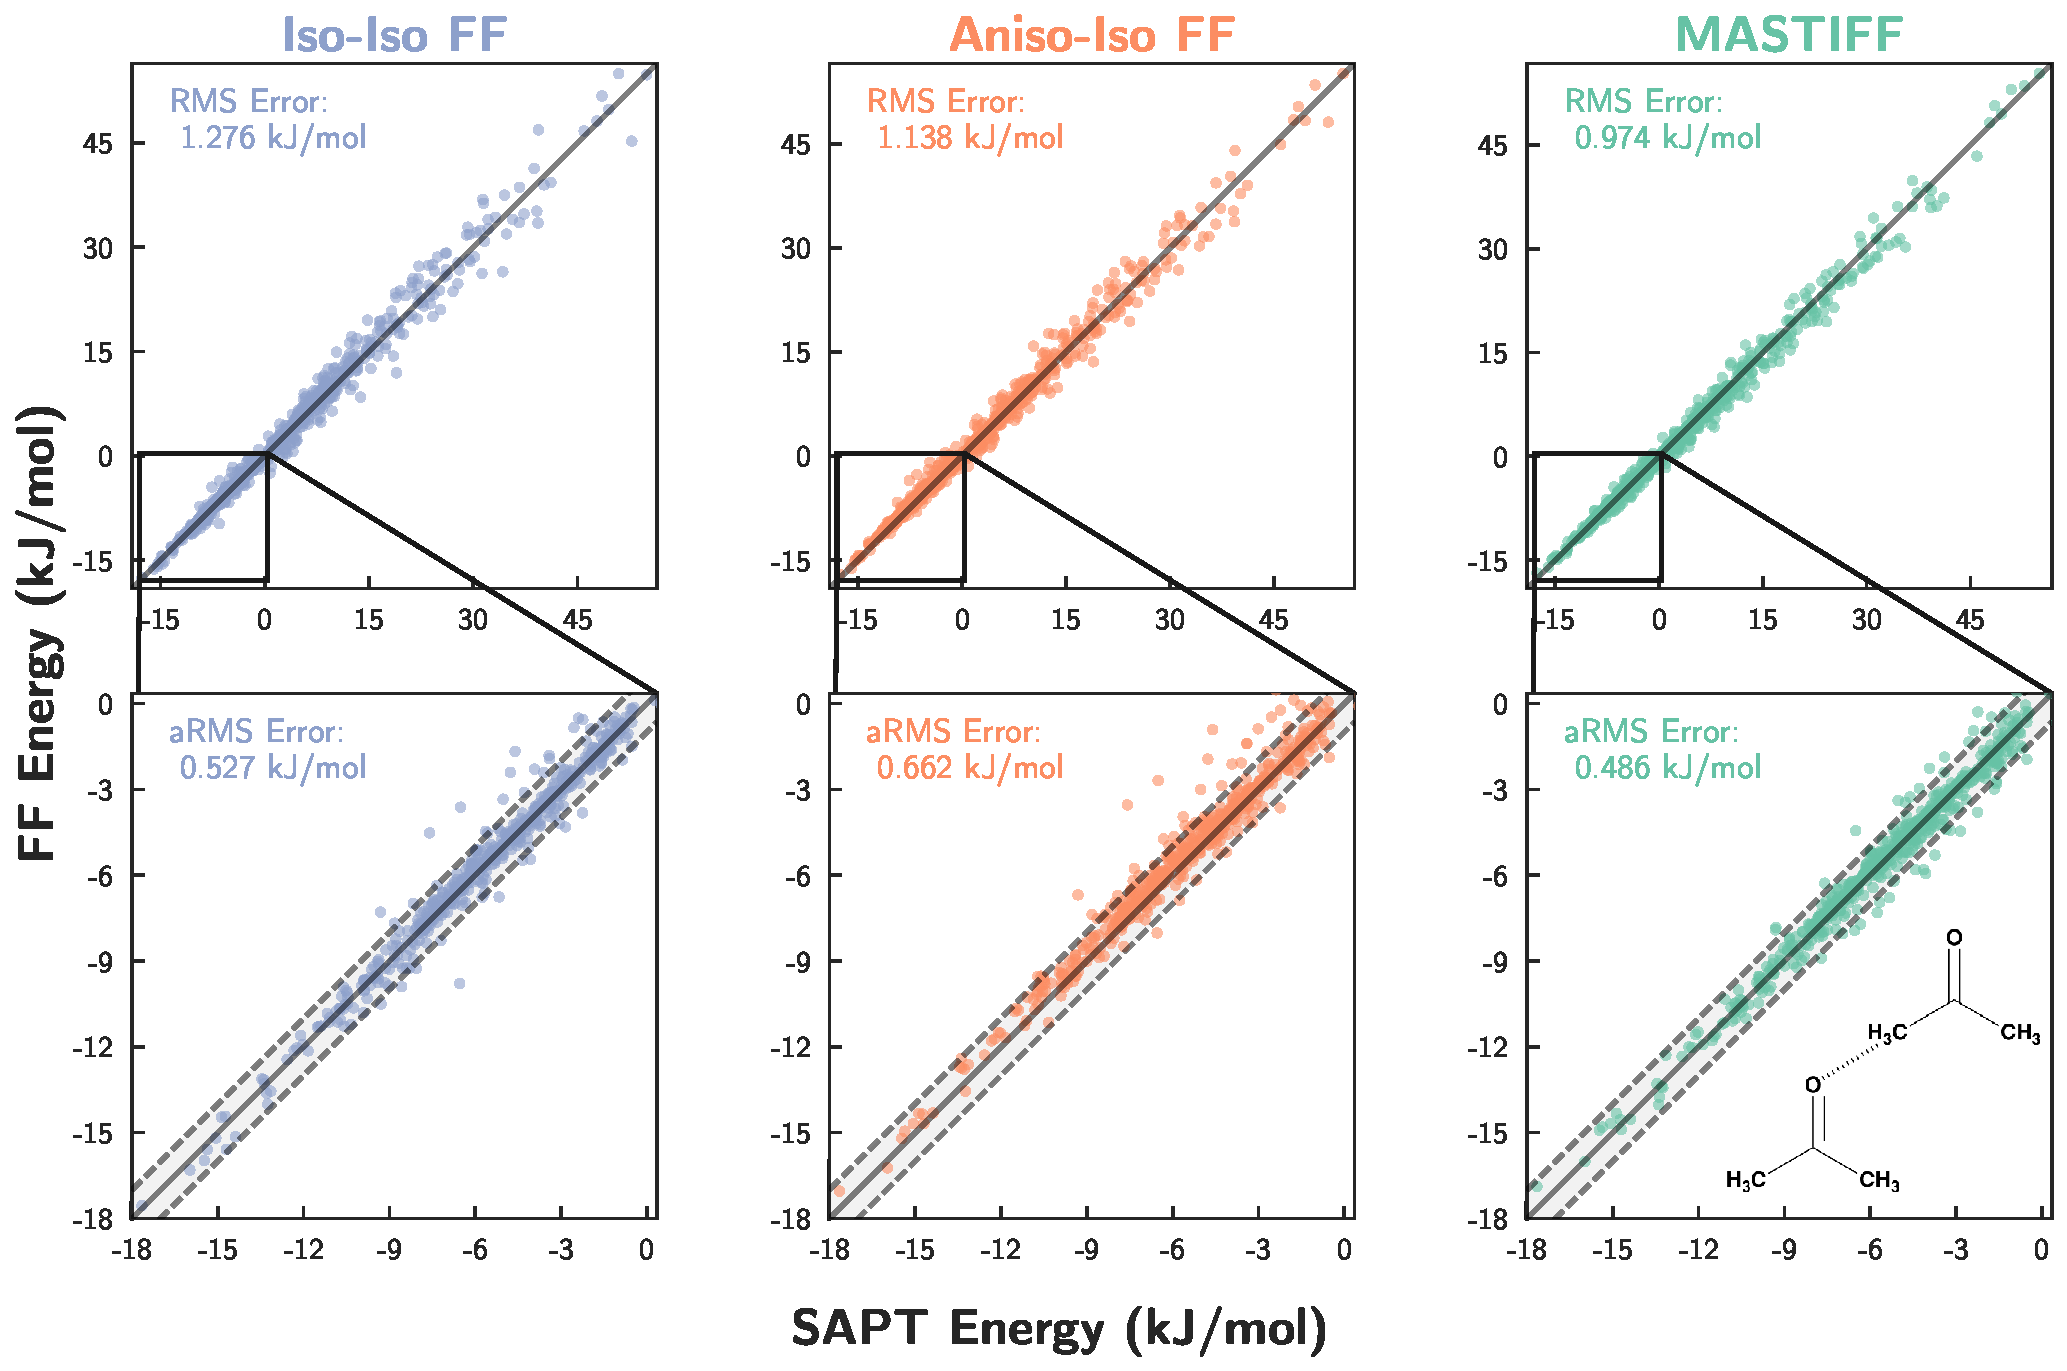
\includegraphics[width=0.9\textwidth]{anisotropic/si/homodimer_figures/acetone_acetone_comparison.pdf}
    \end{subfigure}
    \begin{subfigure}{\textwidth}
        \caption{Ar Dimer}
        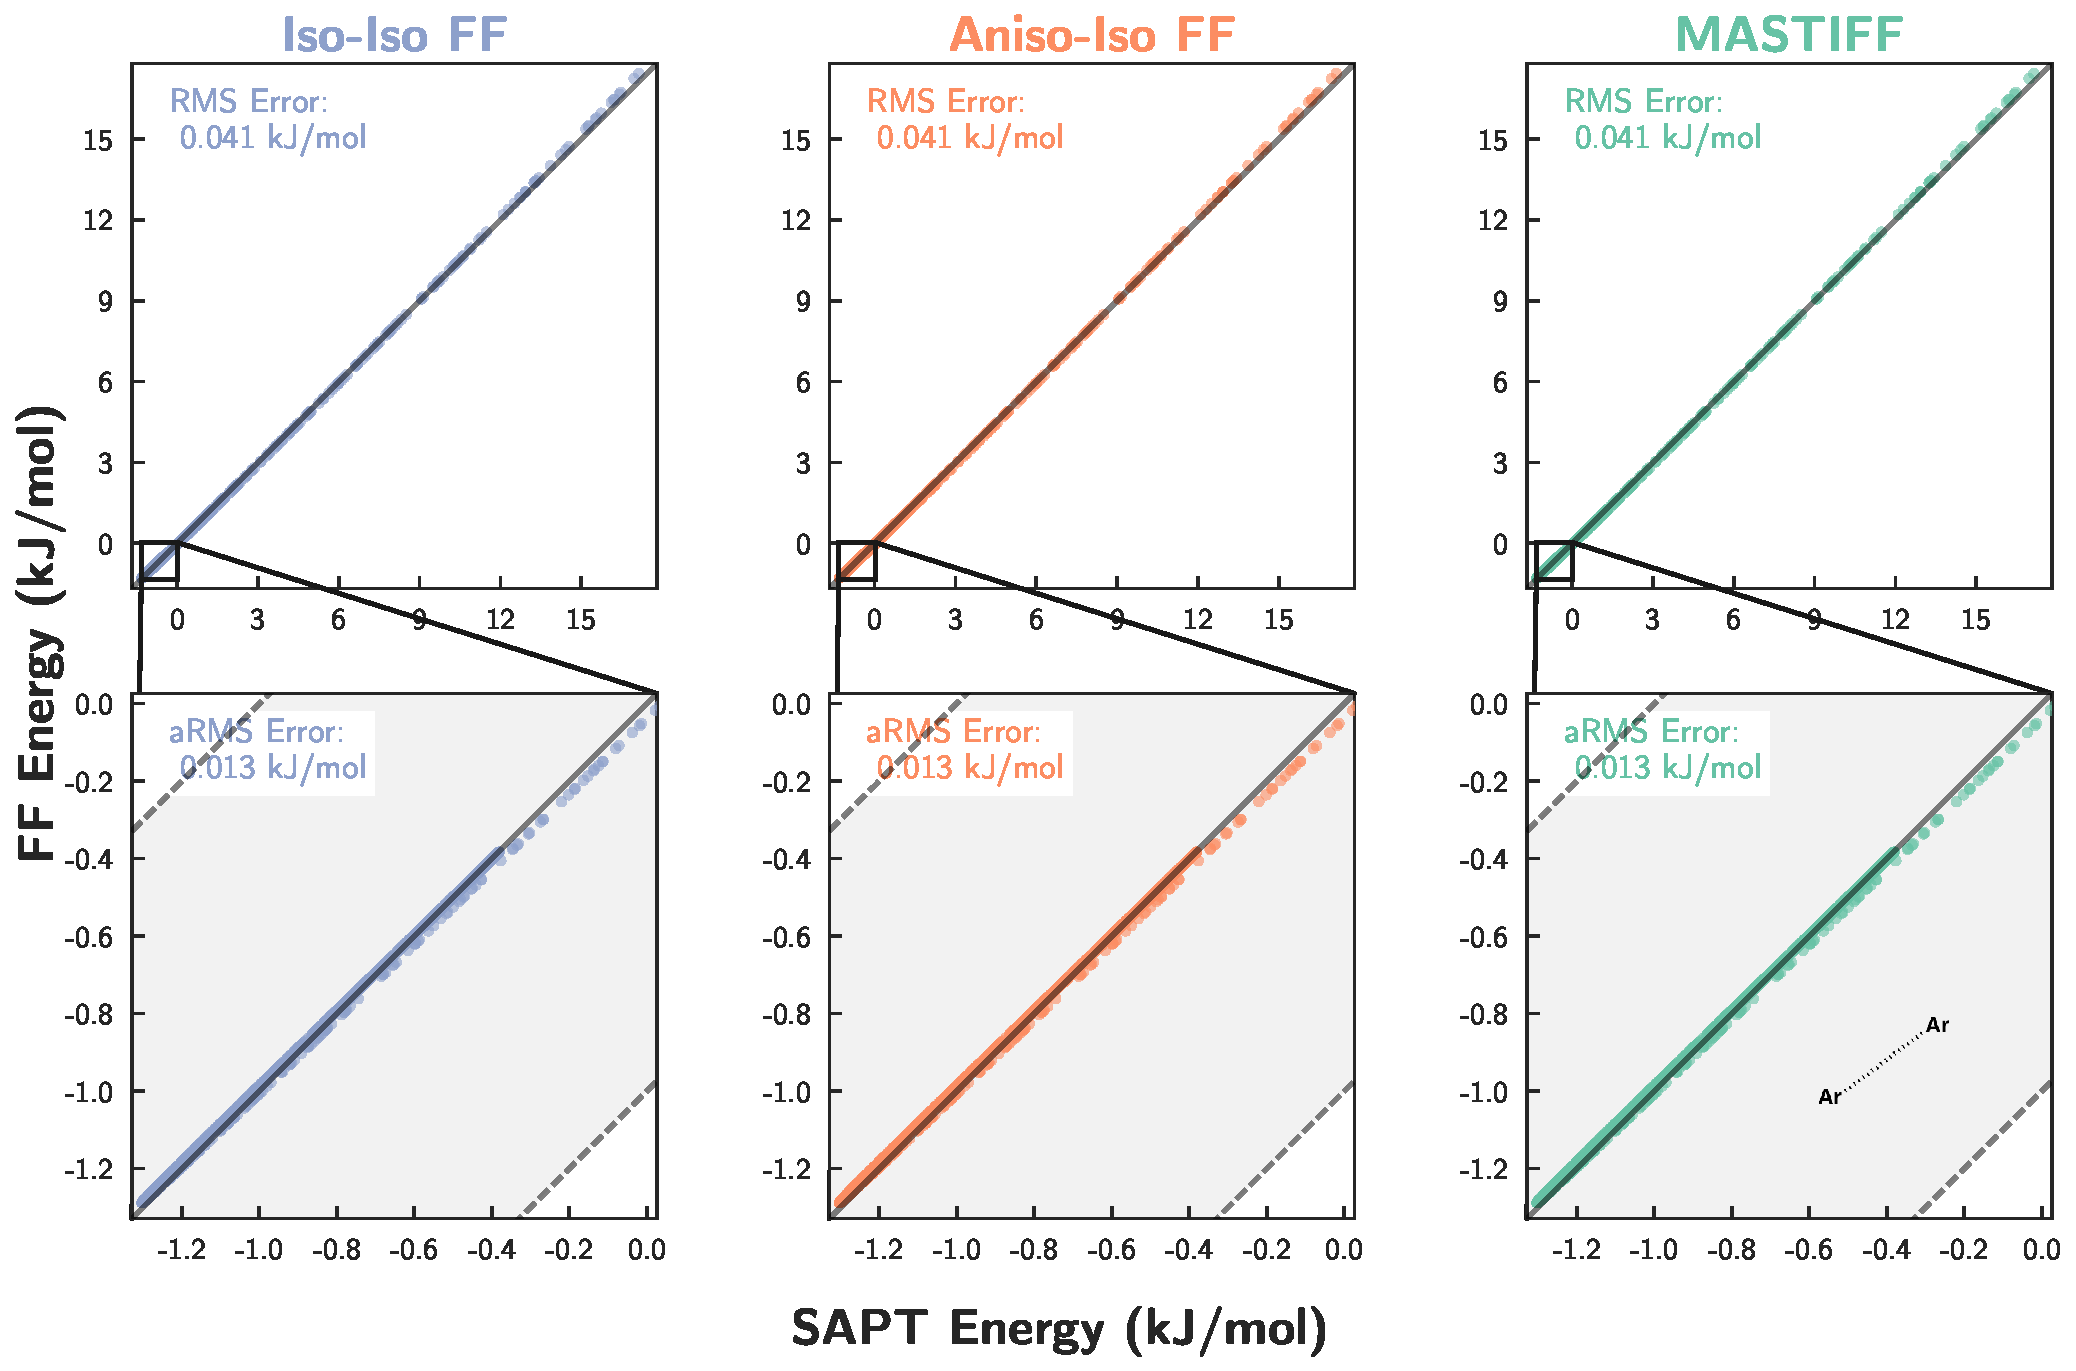
\includegraphics[width=0.9\textwidth]{anisotropic/si/homodimer_figures/ar_ar_comparison.pdf}
    \end{subfigure}
    \end{figure}
    \begin{figure}
    \ContinuedFloat
    \begin{subfigure}{\textwidth}
        \caption{Chloromethane Dimer}
        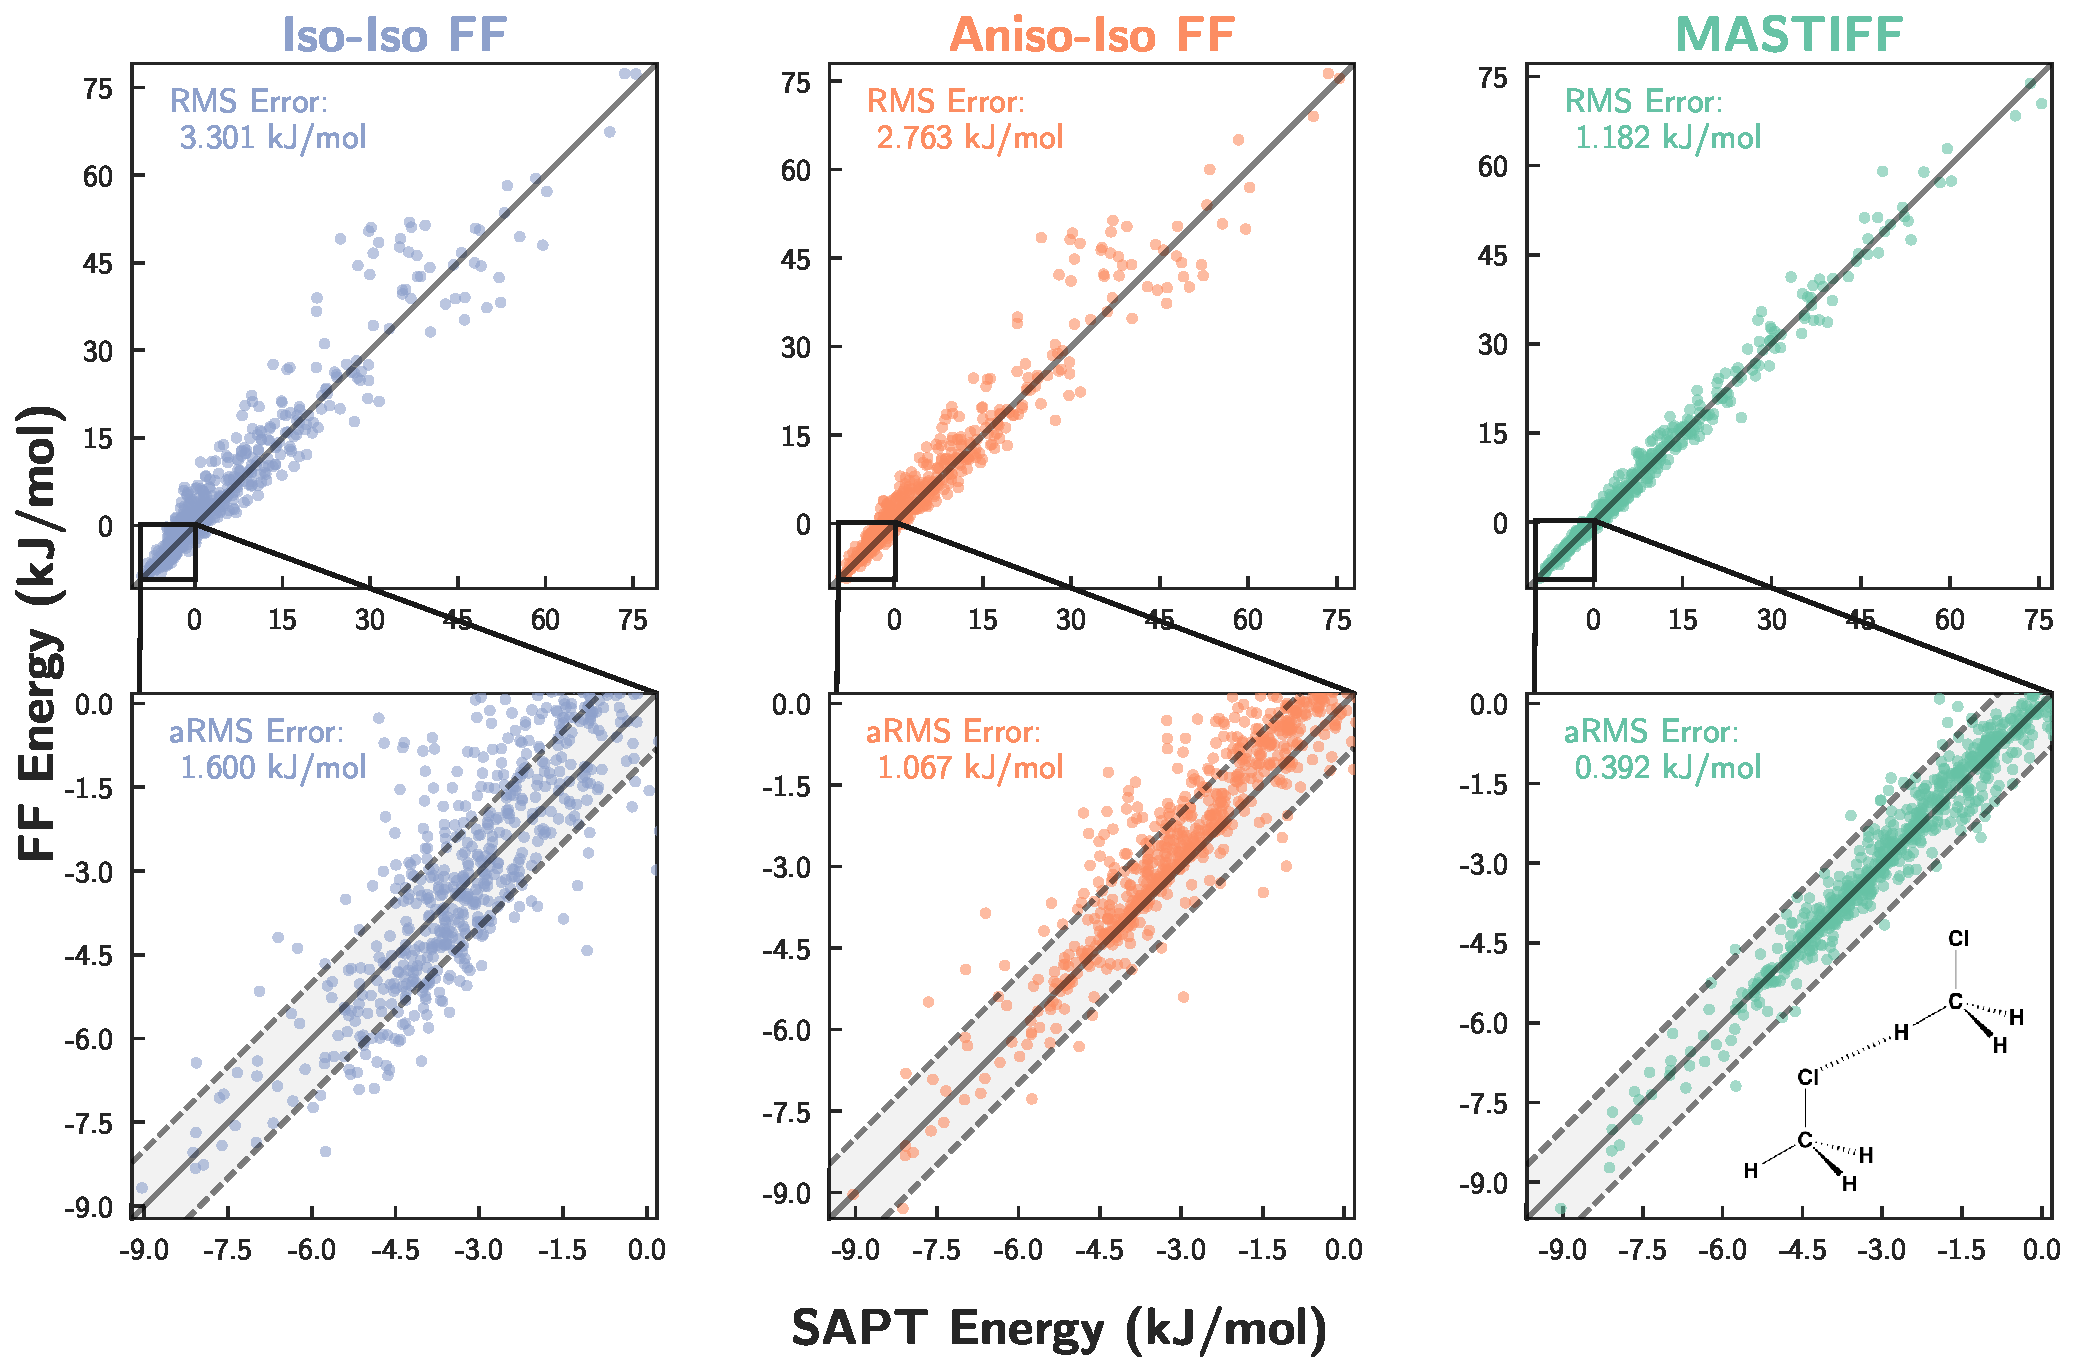
\includegraphics[width=0.9\textwidth]{anisotropic/si/homodimer_figures/chloromethane_chloromethane_comparison.pdf}
    \end{subfigure}
    \begin{subfigure}{\textwidth}
        \caption{\co Dimer}
        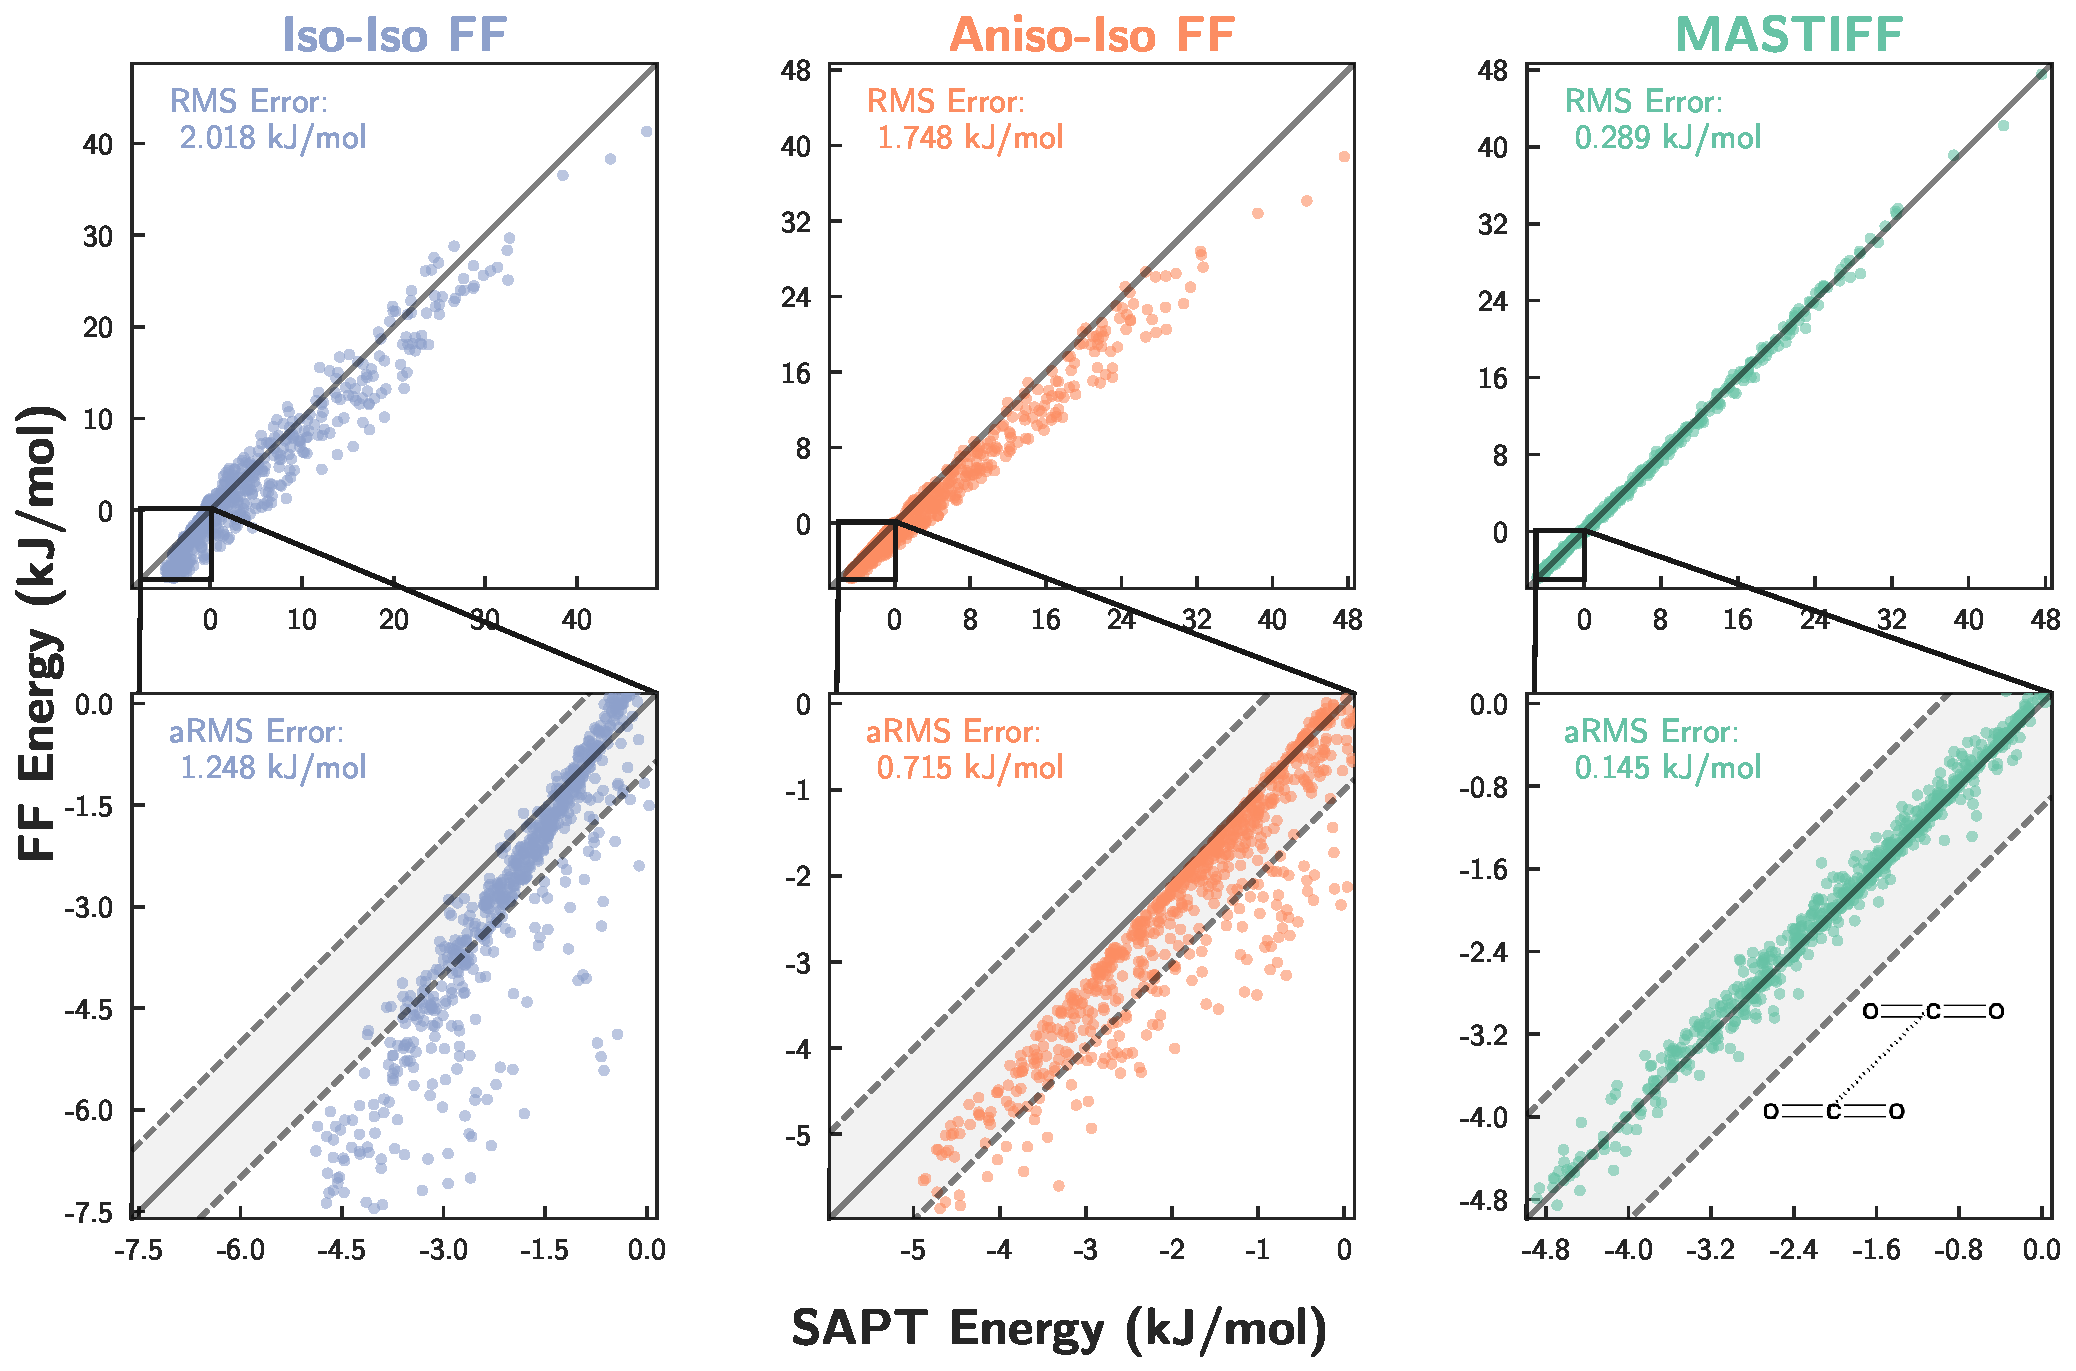
\includegraphics[width=0.9\textwidth]{anisotropic/si/homodimer_figures/co2_co2_comparison.pdf}
    \end{subfigure}
    \end{figure}
    \begin{figure}
    \ContinuedFloat
    \begin{subfigure}{\textwidth}
        \caption{Dimethyl Ether Dimer}
        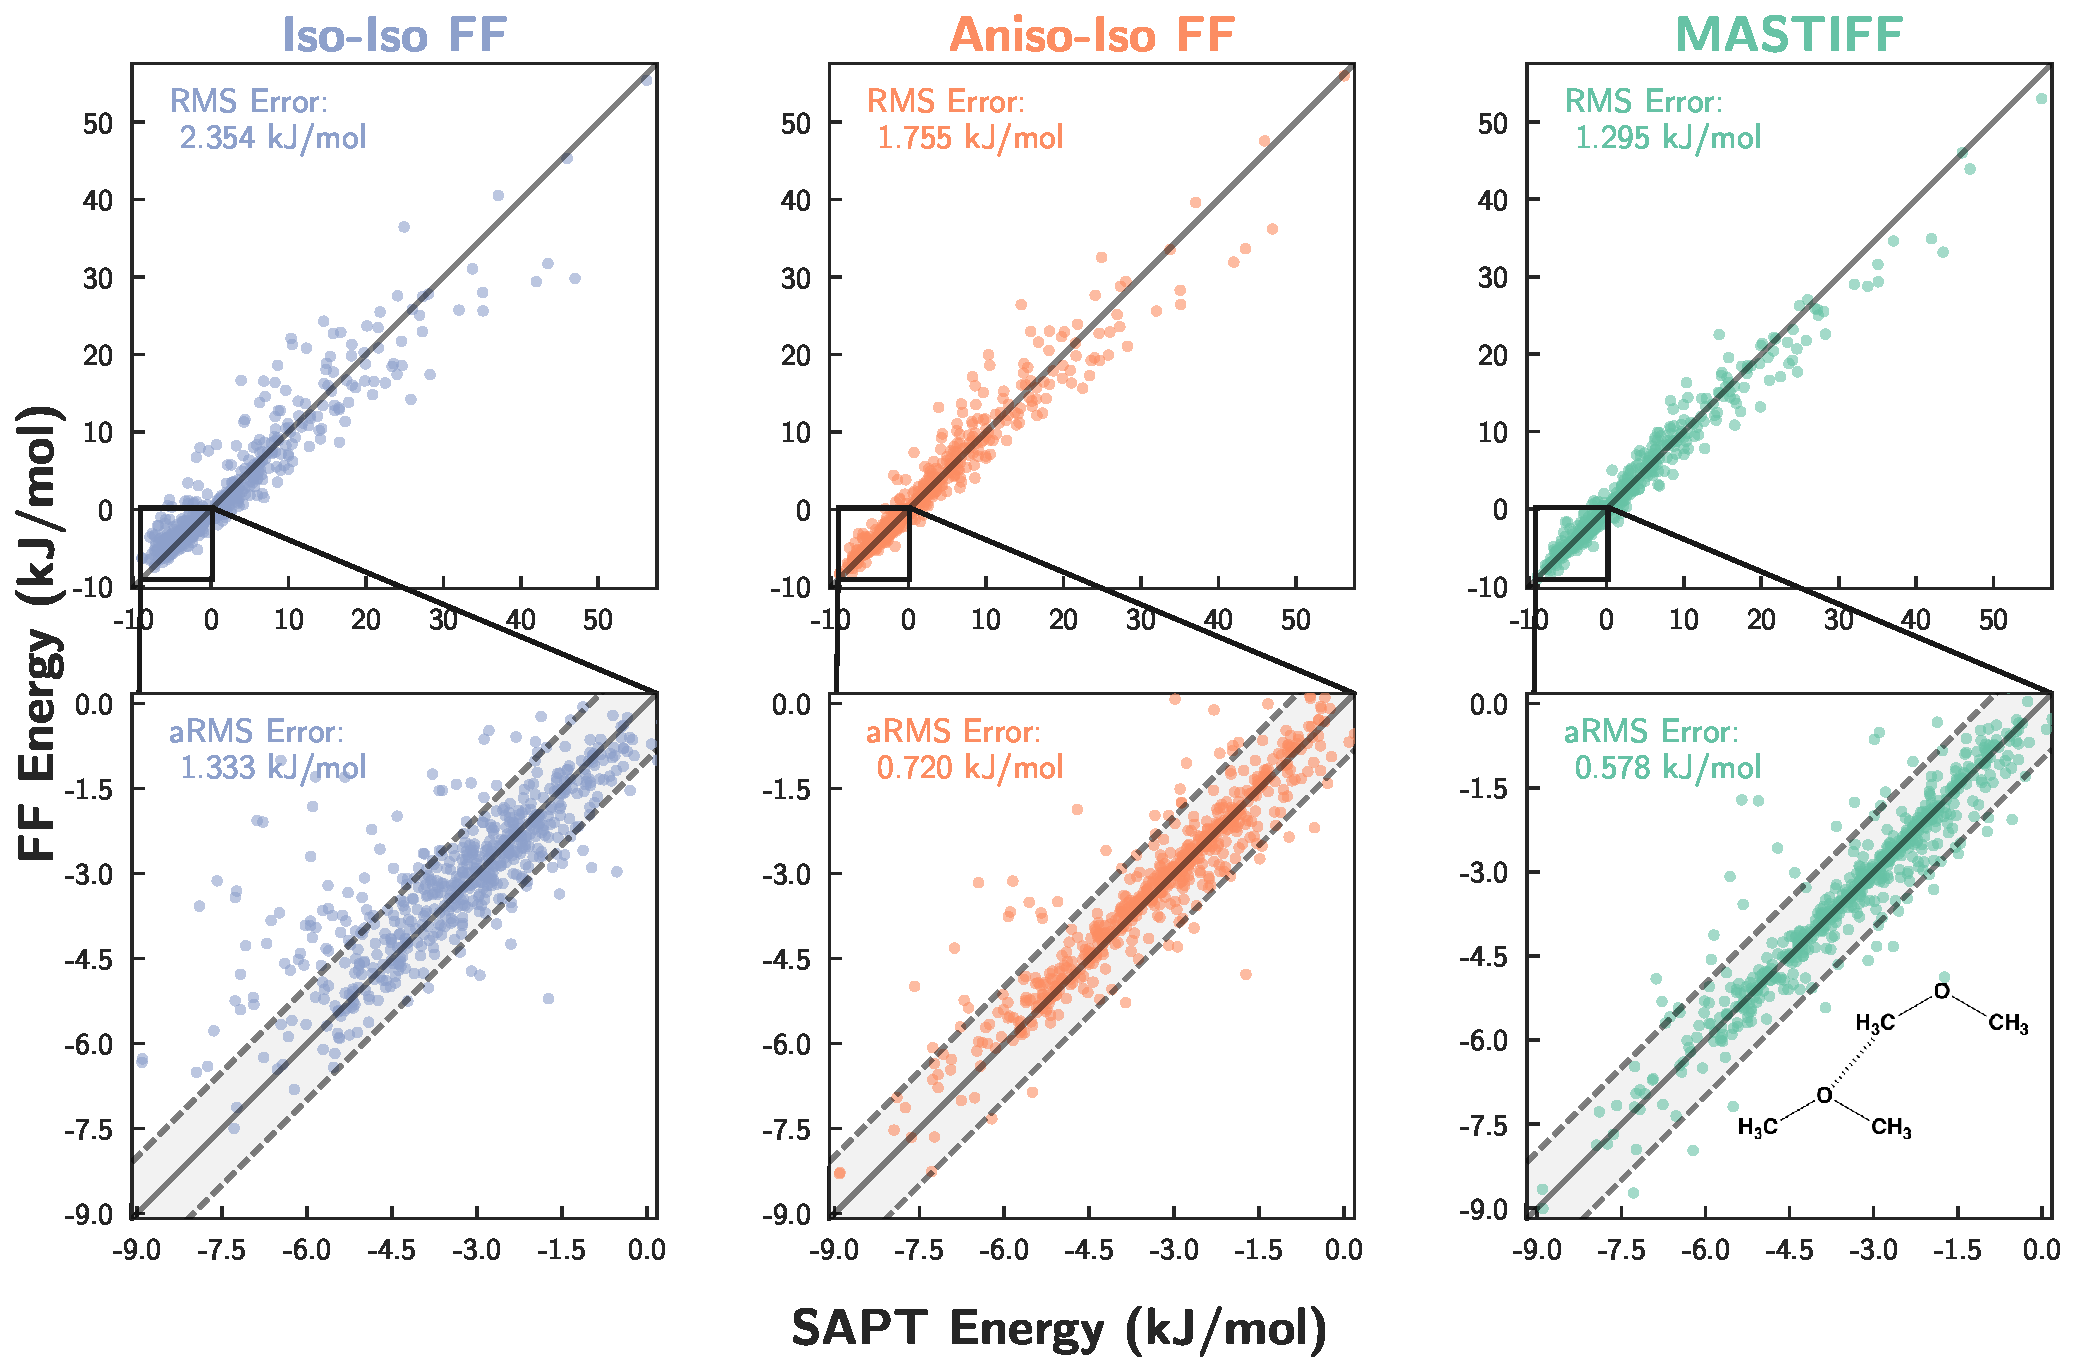
\includegraphics[width=0.9\textwidth]{anisotropic/si/homodimer_figures/dimethyl_ether_dimethyl_ether_comparison.pdf}
    \end{subfigure}
    \begin{subfigure}{\textwidth}
        \caption{Ethane Dimer}
        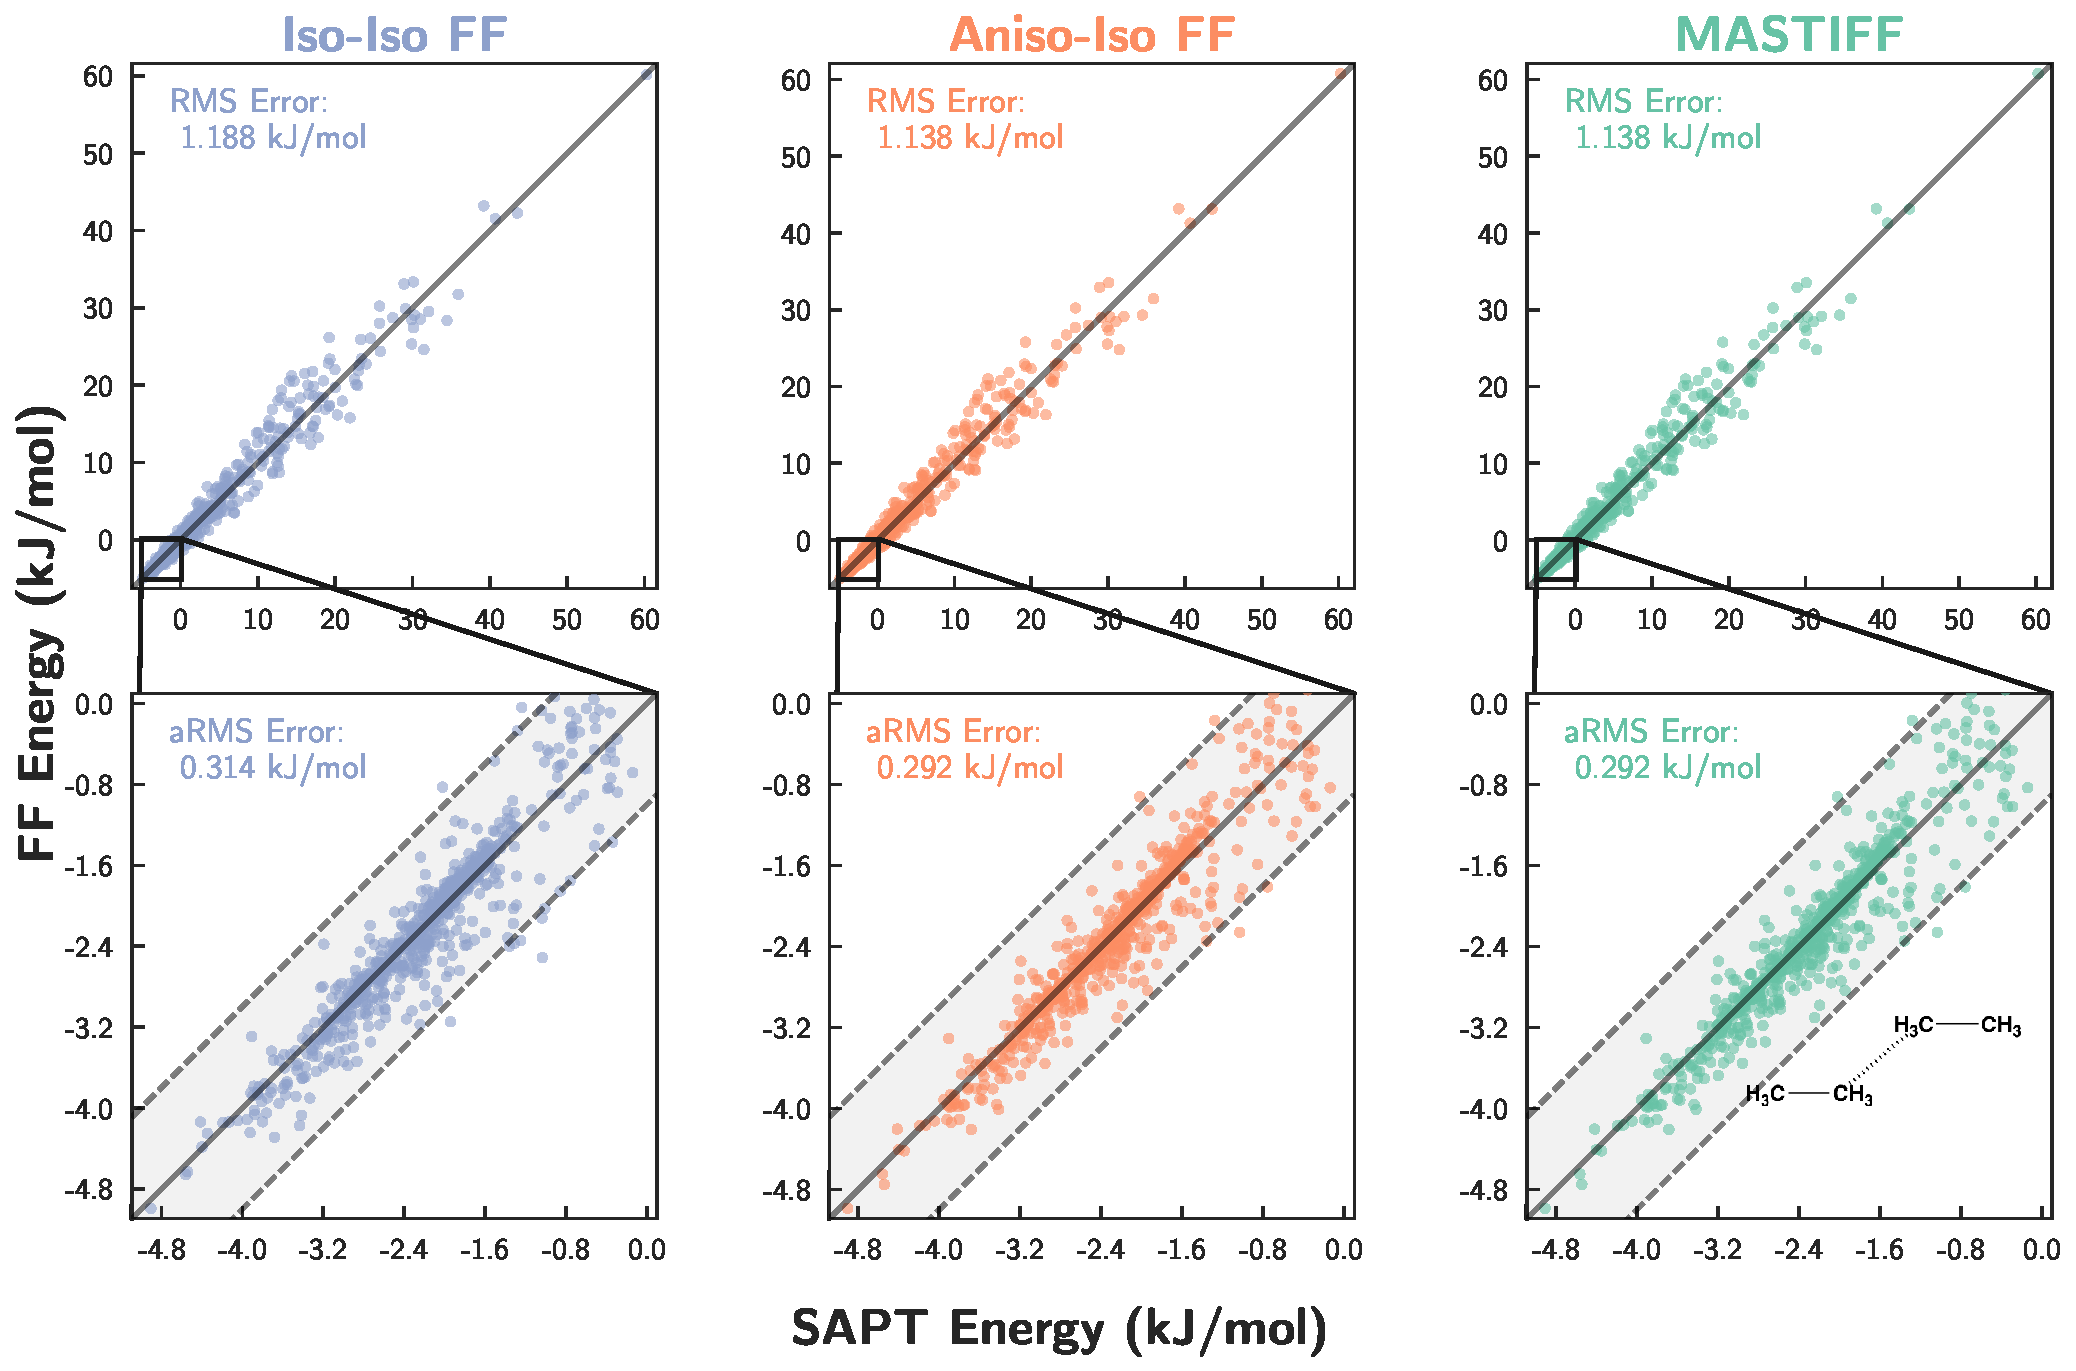
\includegraphics[width=0.9\textwidth]{anisotropic/si/homodimer_figures/ethane_ethane_comparison.pdf}
    \end{subfigure}
    \end{figure}
    \begin{figure}
    \ContinuedFloat
    \begin{subfigure}{\textwidth}
        \caption{Ethanol Dimer}
        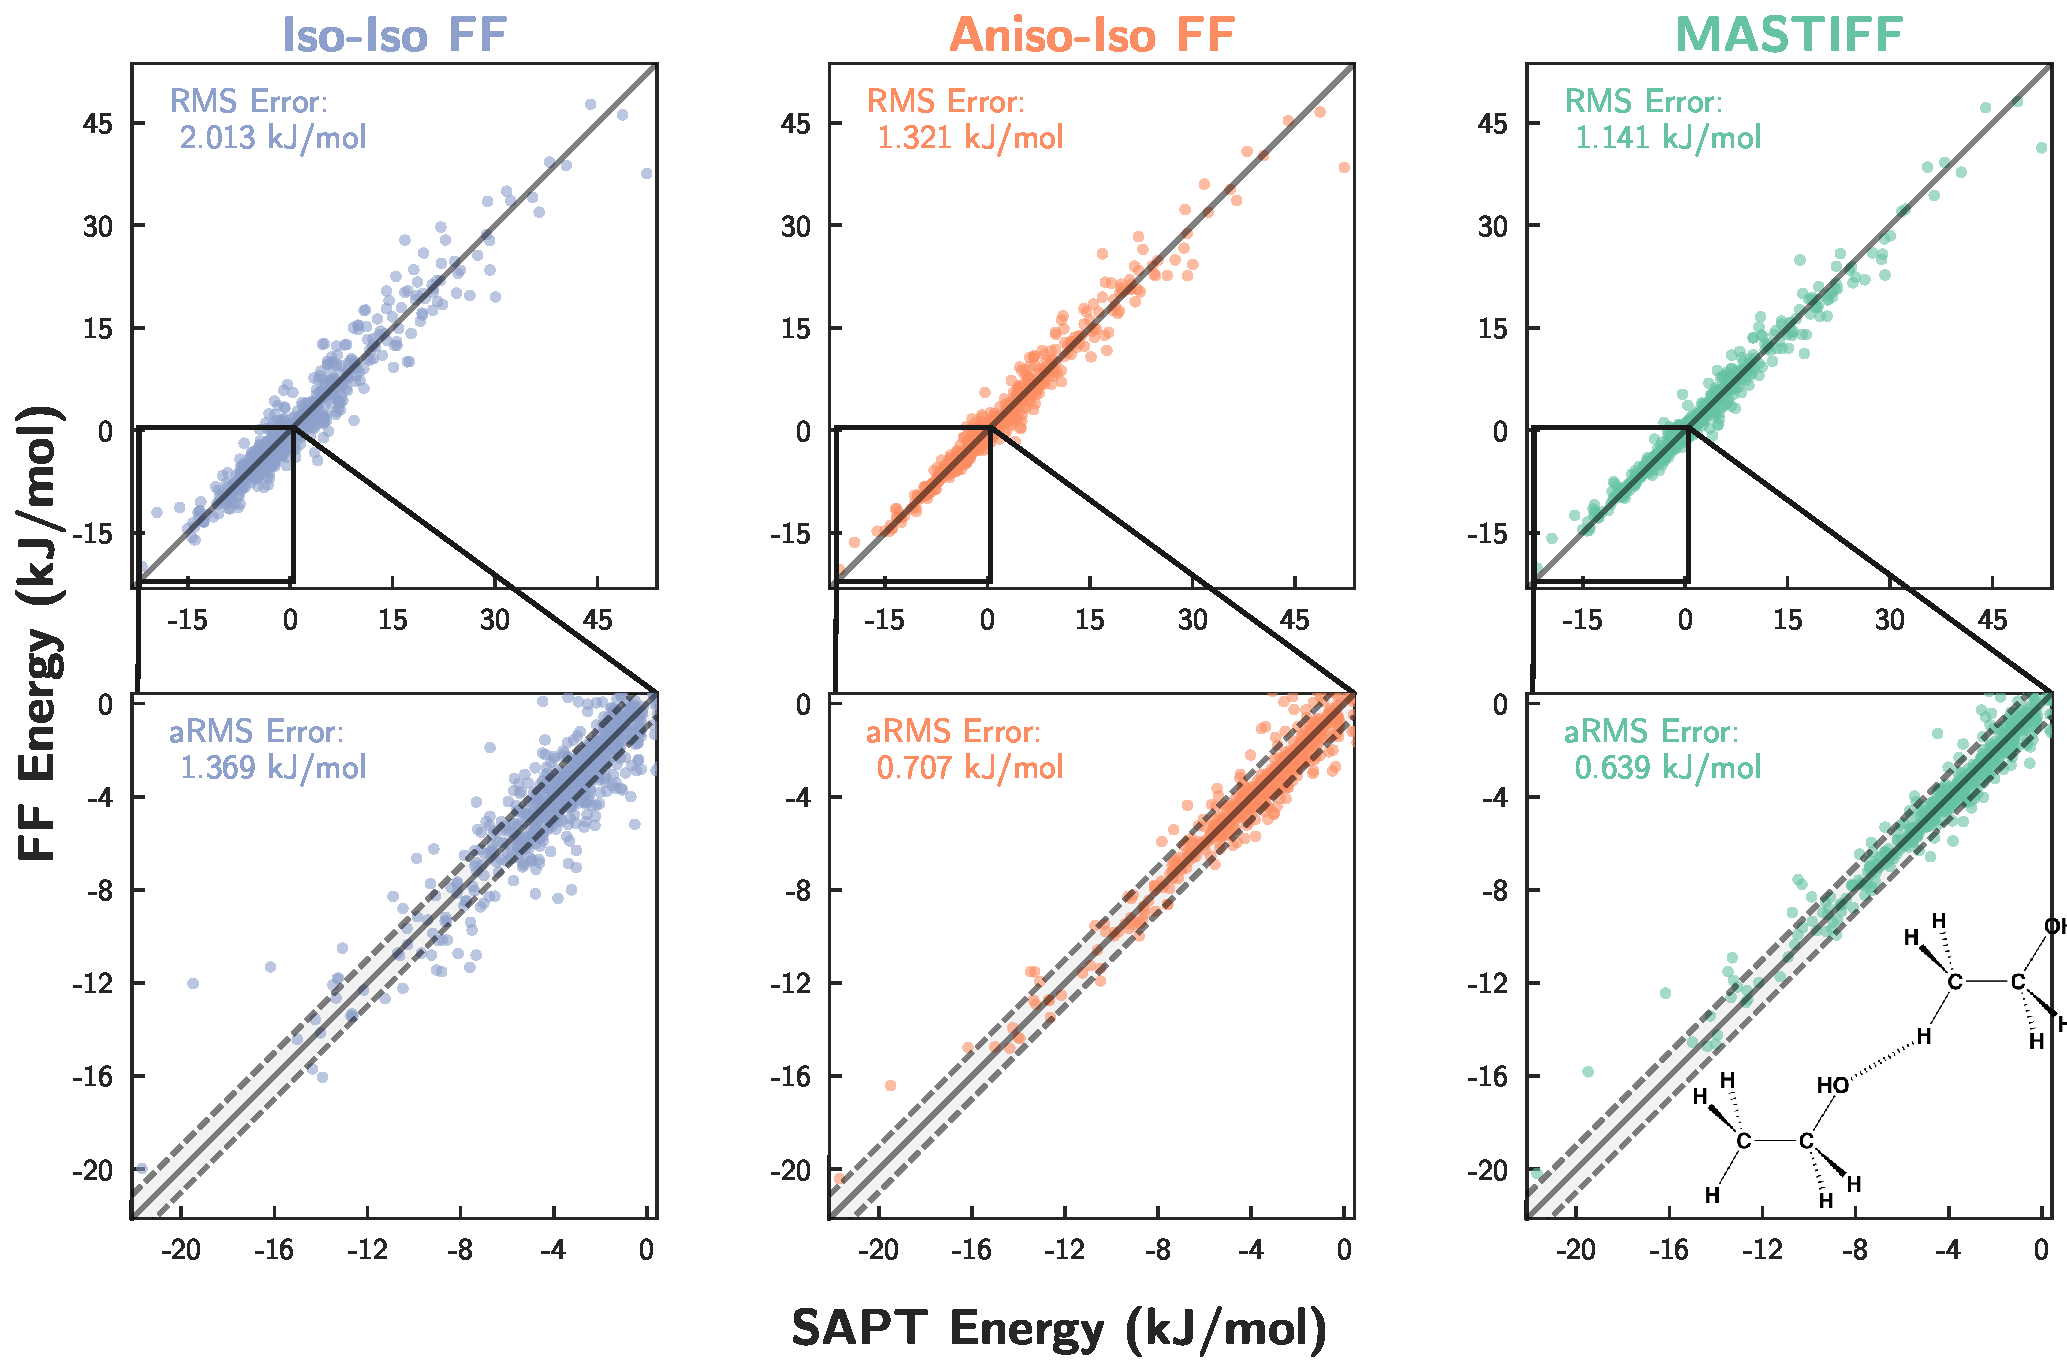
\includegraphics[width=0.9\textwidth]{anisotropic/si/homodimer_figures/ethanol_ethanol_comparison.pdf}
    \end{subfigure}
    \begin{subfigure}{\textwidth}
        \caption{Ethene Dimer}
        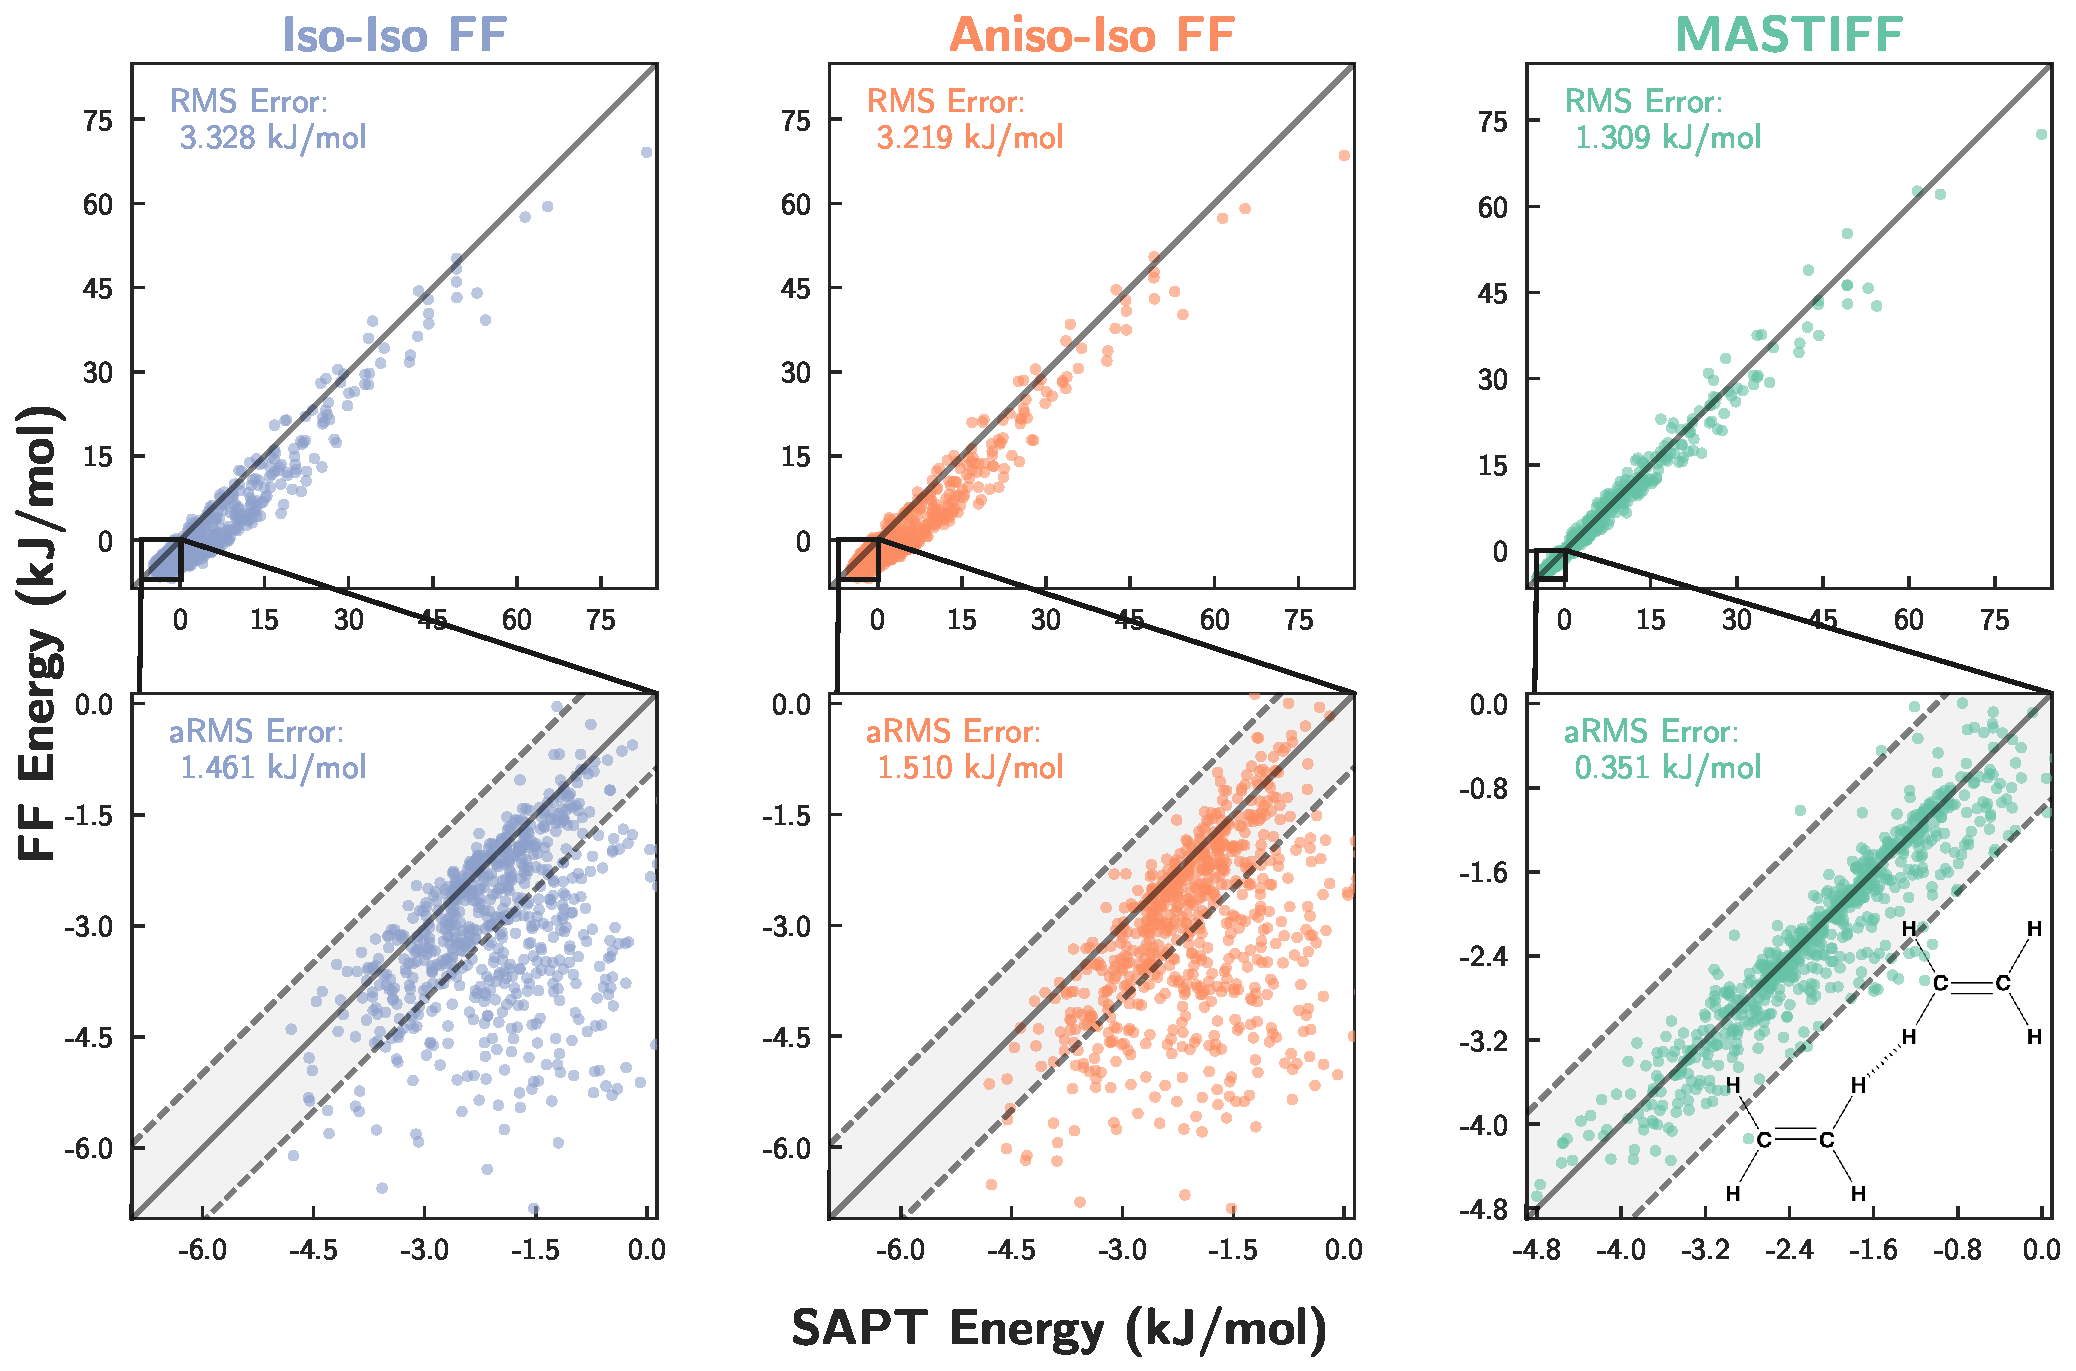
\includegraphics[width=0.9\textwidth]{anisotropic/si/homodimer_figures/ethene_ethene_comparison.pdf}
    \end{subfigure}
    \end{figure}
    \begin{figure}
    \ContinuedFloat
    \begin{subfigure}{\textwidth}
        \caption{\ho Dimer}
        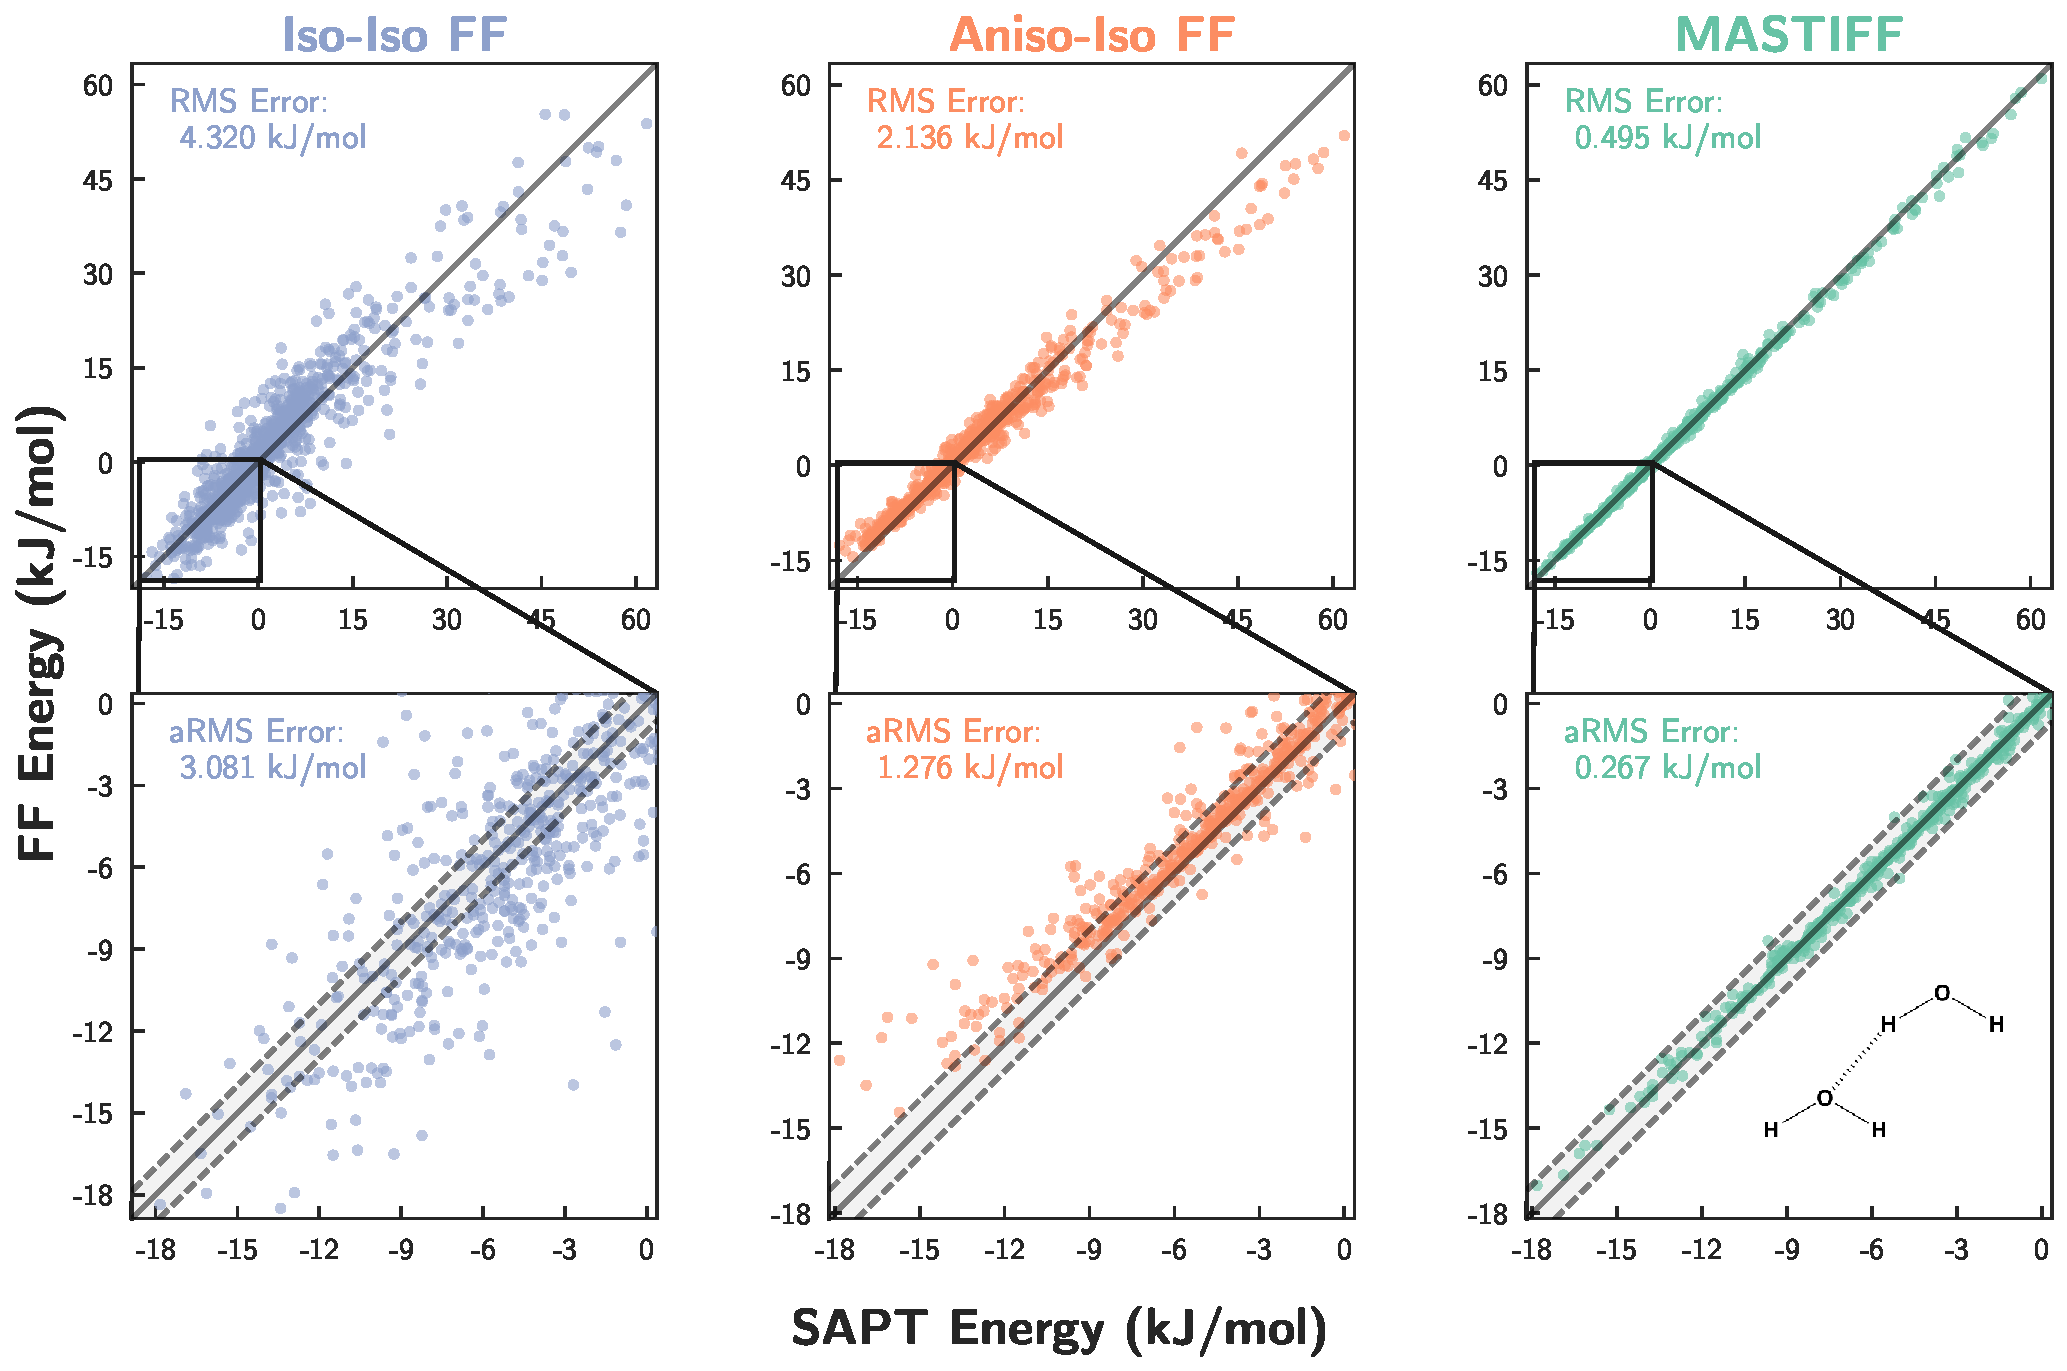
\includegraphics[width=0.9\textwidth]{anisotropic/si/homodimer_figures/h2o_h2o_comparison.pdf}
    \end{subfigure}
    \begin{subfigure}{\textwidth}
        \caption{Methane Dimer}
        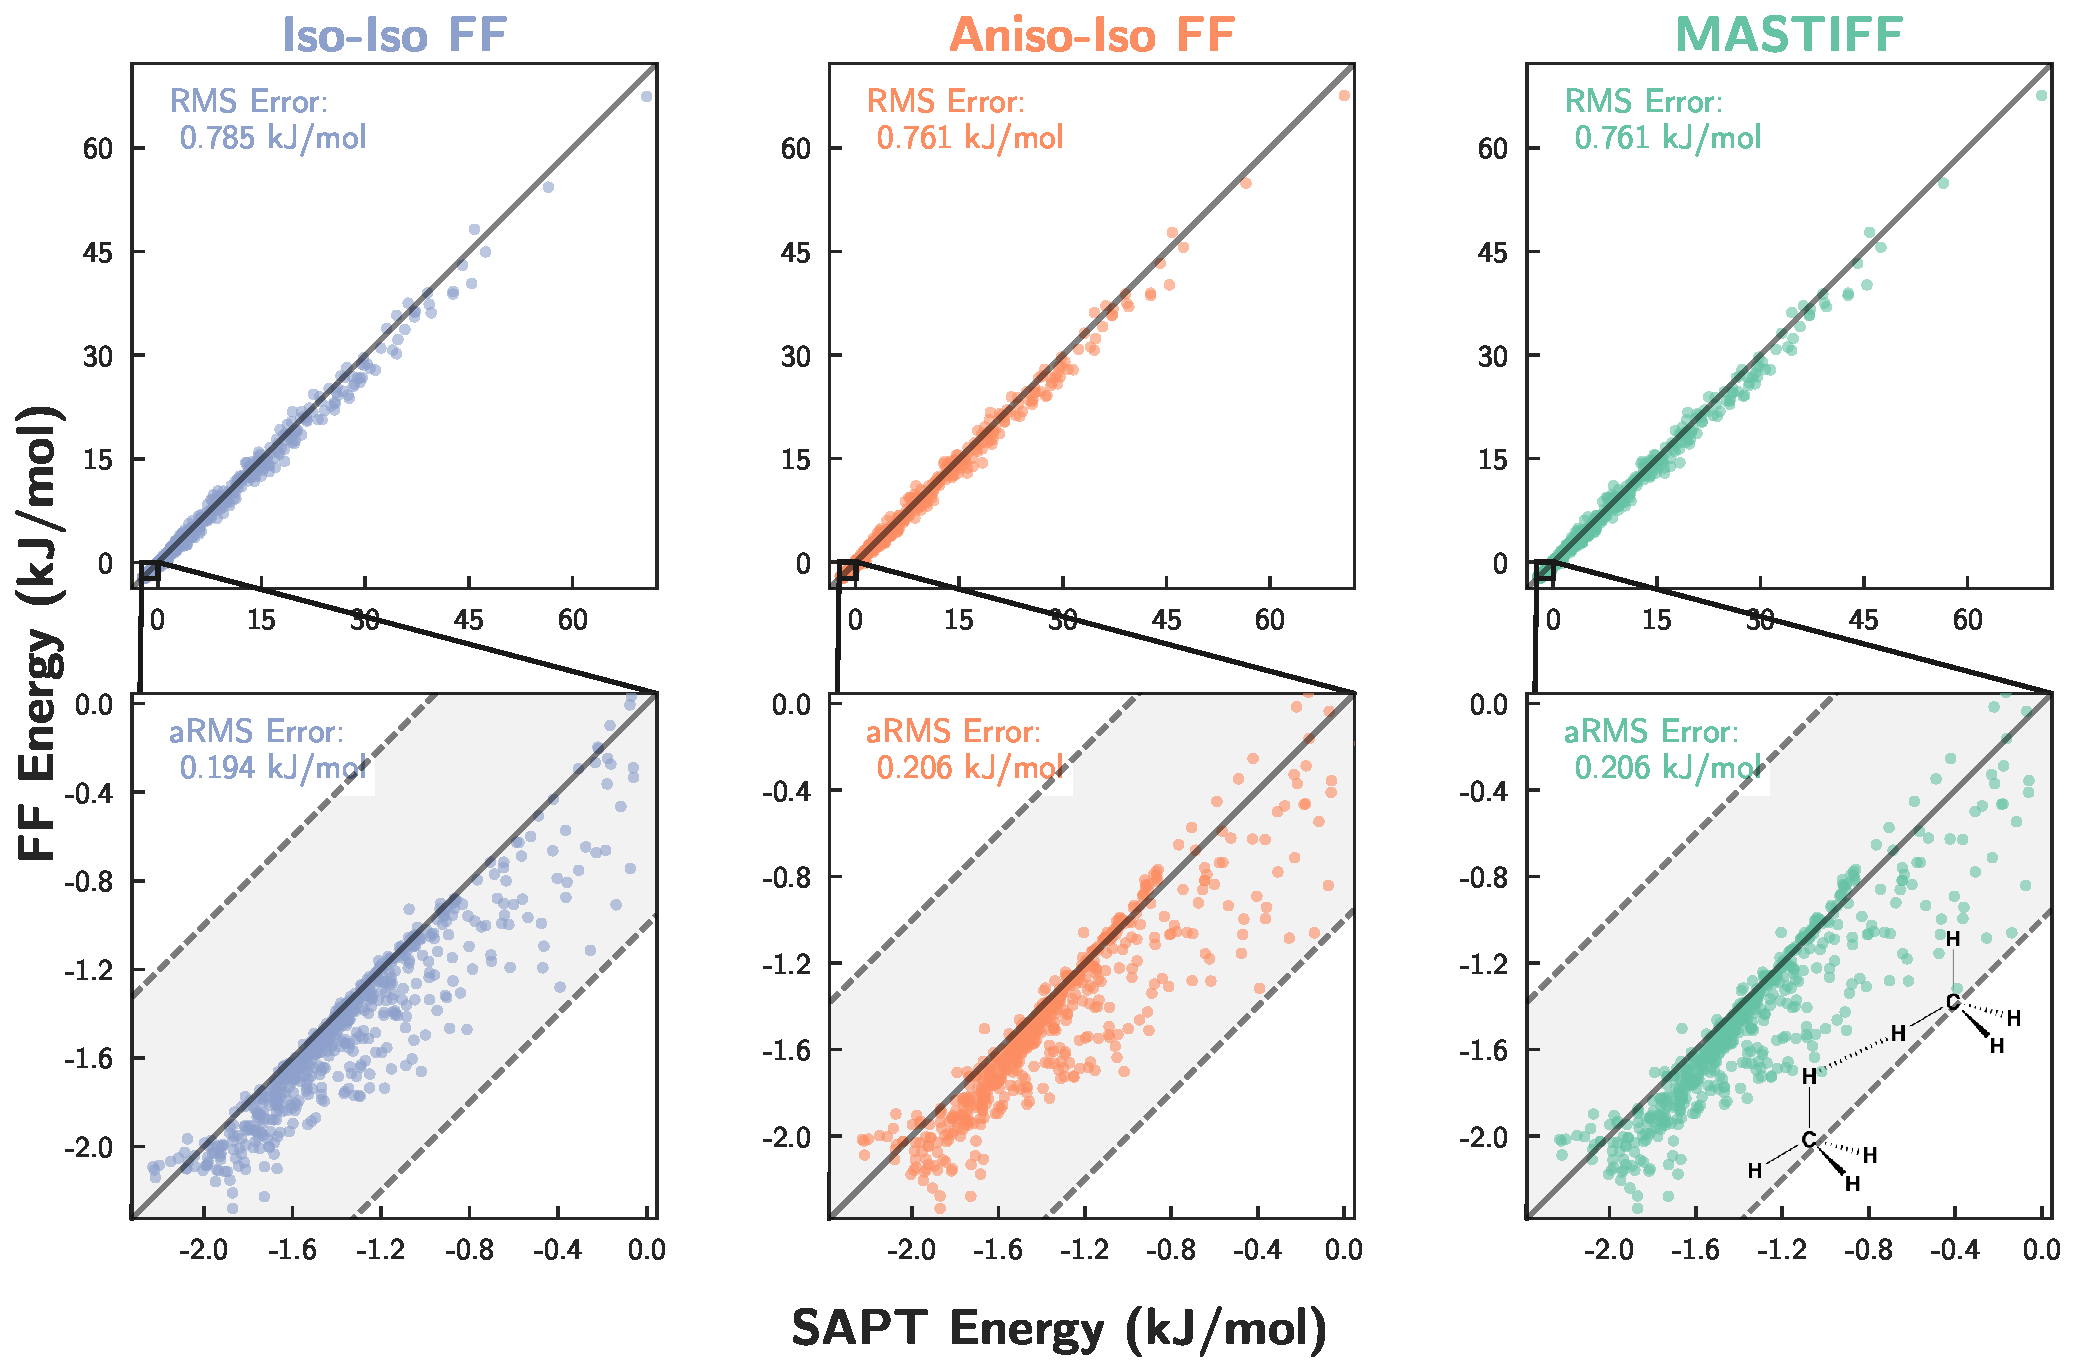
\includegraphics[width=0.9\textwidth]{anisotropic/si/homodimer_figures/methane_methane_comparison.pdf}
    \end{subfigure}
    \end{figure}
    \begin{figure}
    \ContinuedFloat
    \begin{subfigure}{\textwidth}
        \caption{Methanol Dimer}
        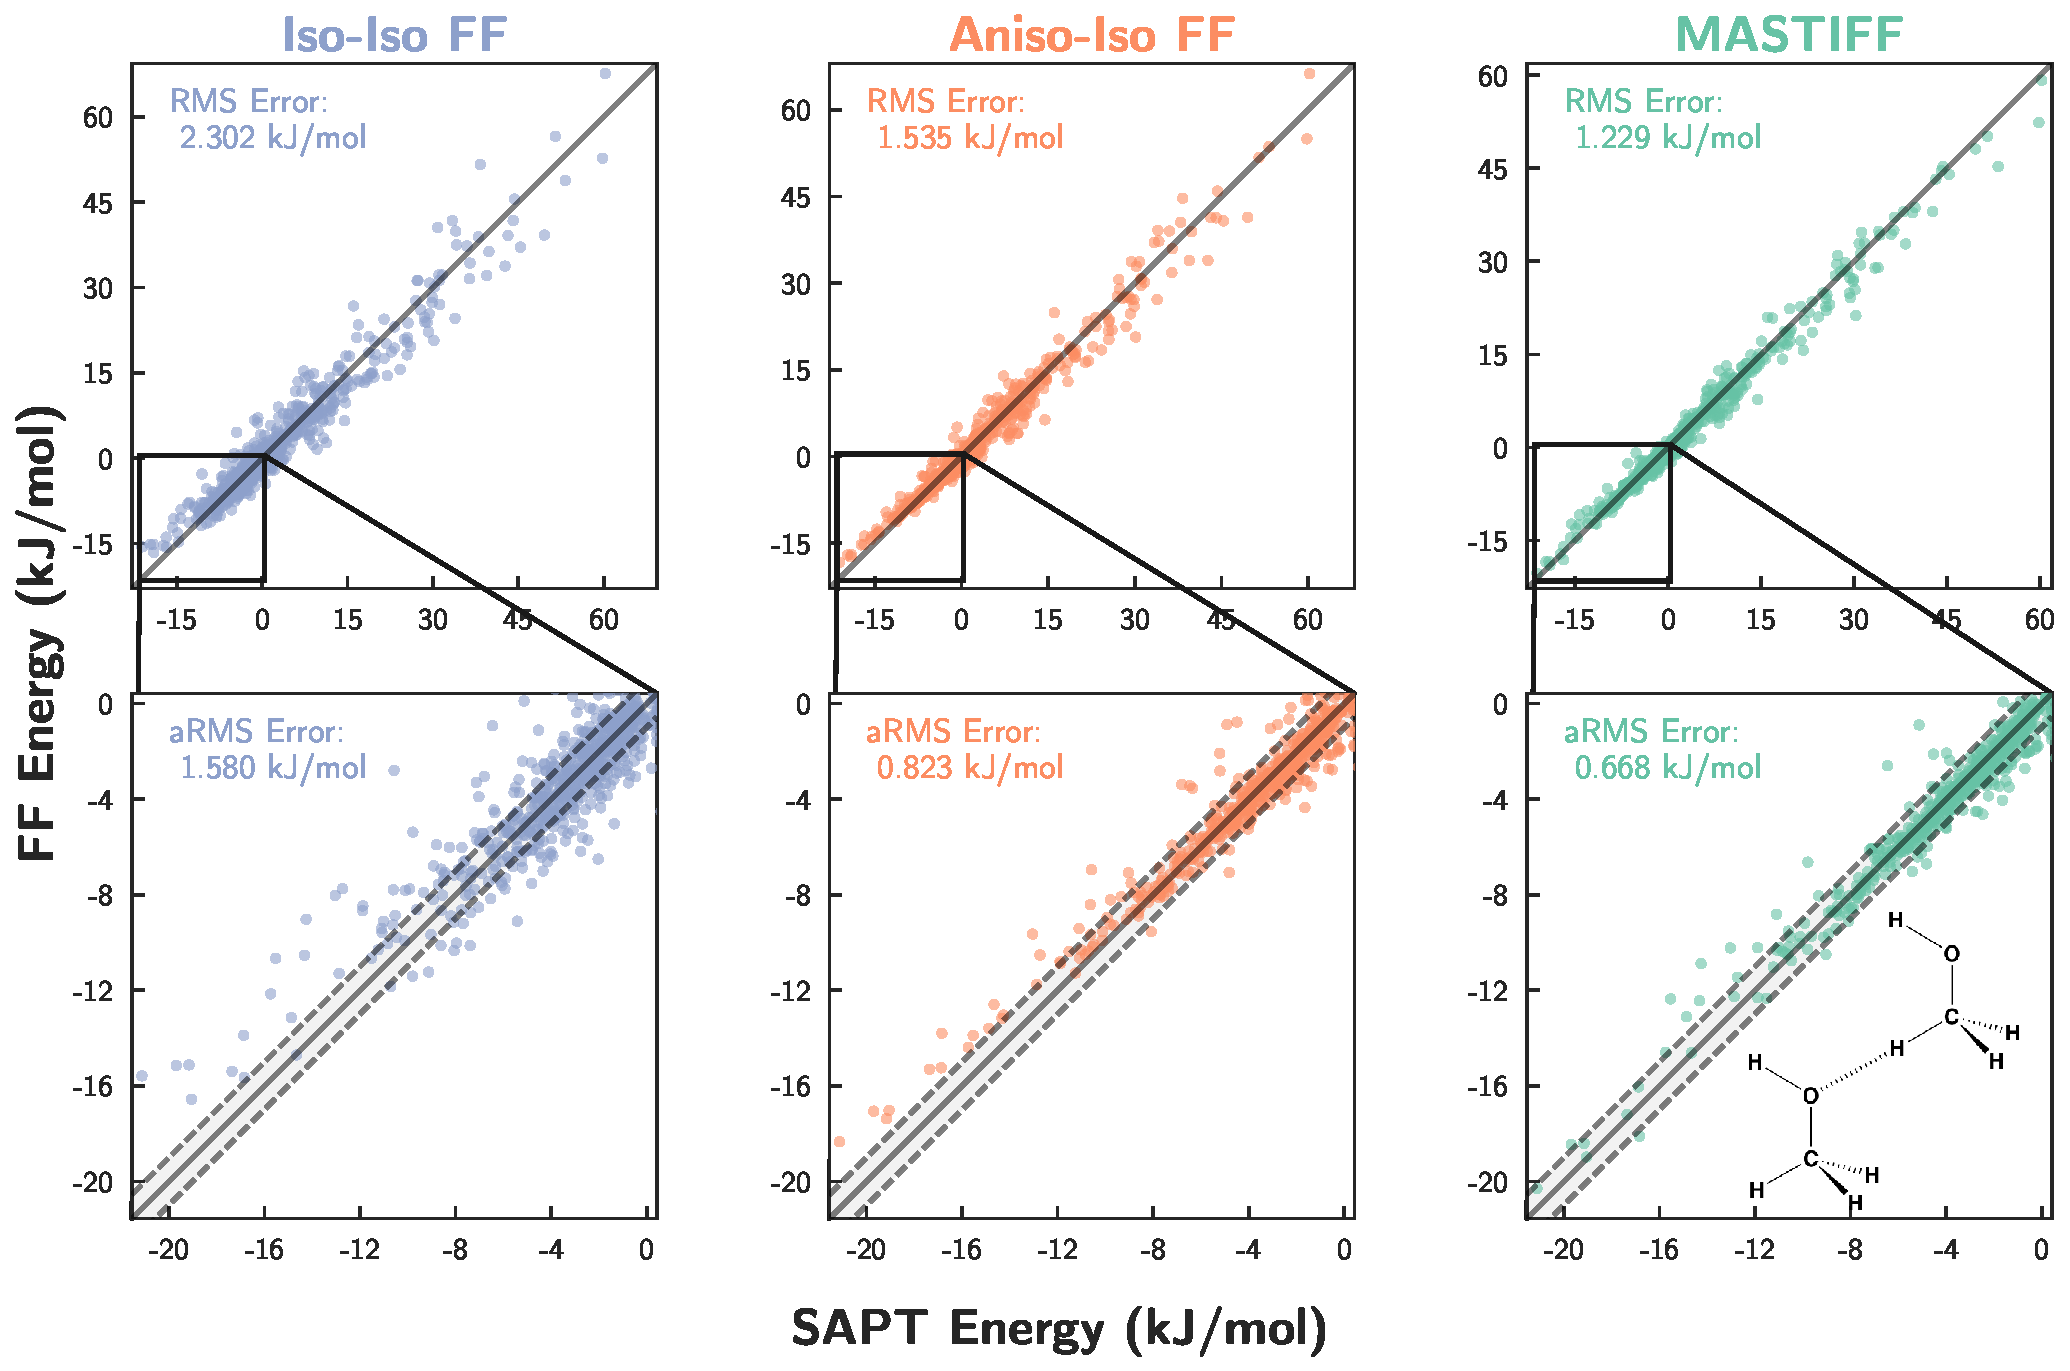
\includegraphics[width=0.9\textwidth]{anisotropic/si/homodimer_figures/methanol_methanol_comparison.pdf}
    \end{subfigure}
    \begin{subfigure}{\textwidth}
        \caption{Methyl Amine Dimer}
        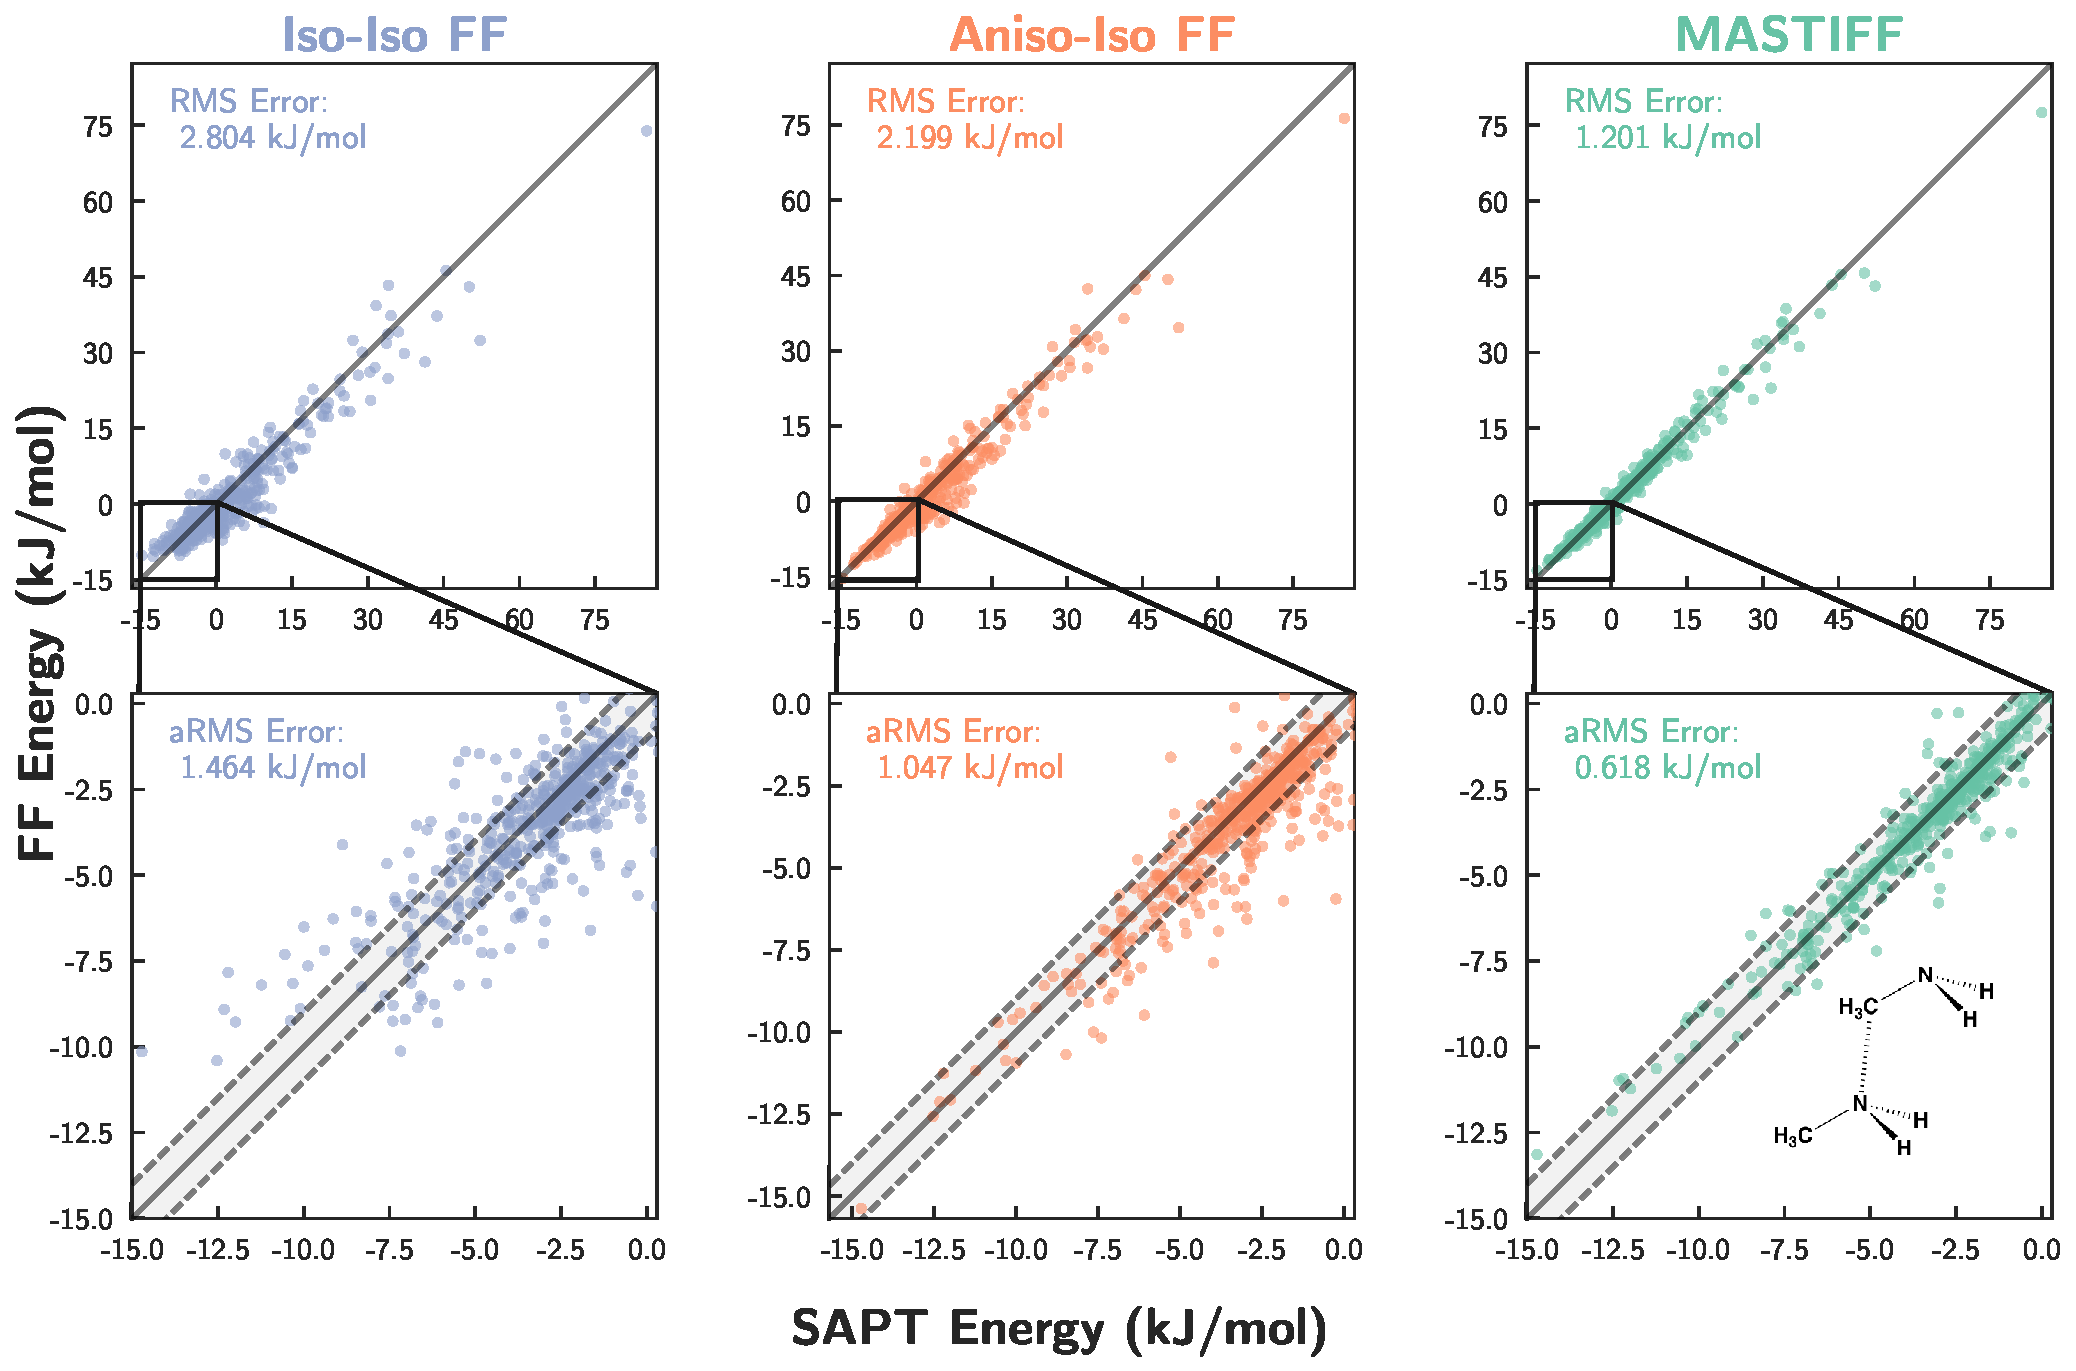
\includegraphics[width=0.9\textwidth]{anisotropic/si/homodimer_figures/methyl_amine_methyl_amine_comparison.pdf}
    \end{subfigure}
    \end{figure}
    \begin{figure}
    \ContinuedFloat
    \begin{subfigure}{\textwidth}
        \caption{\nh Dimer}
        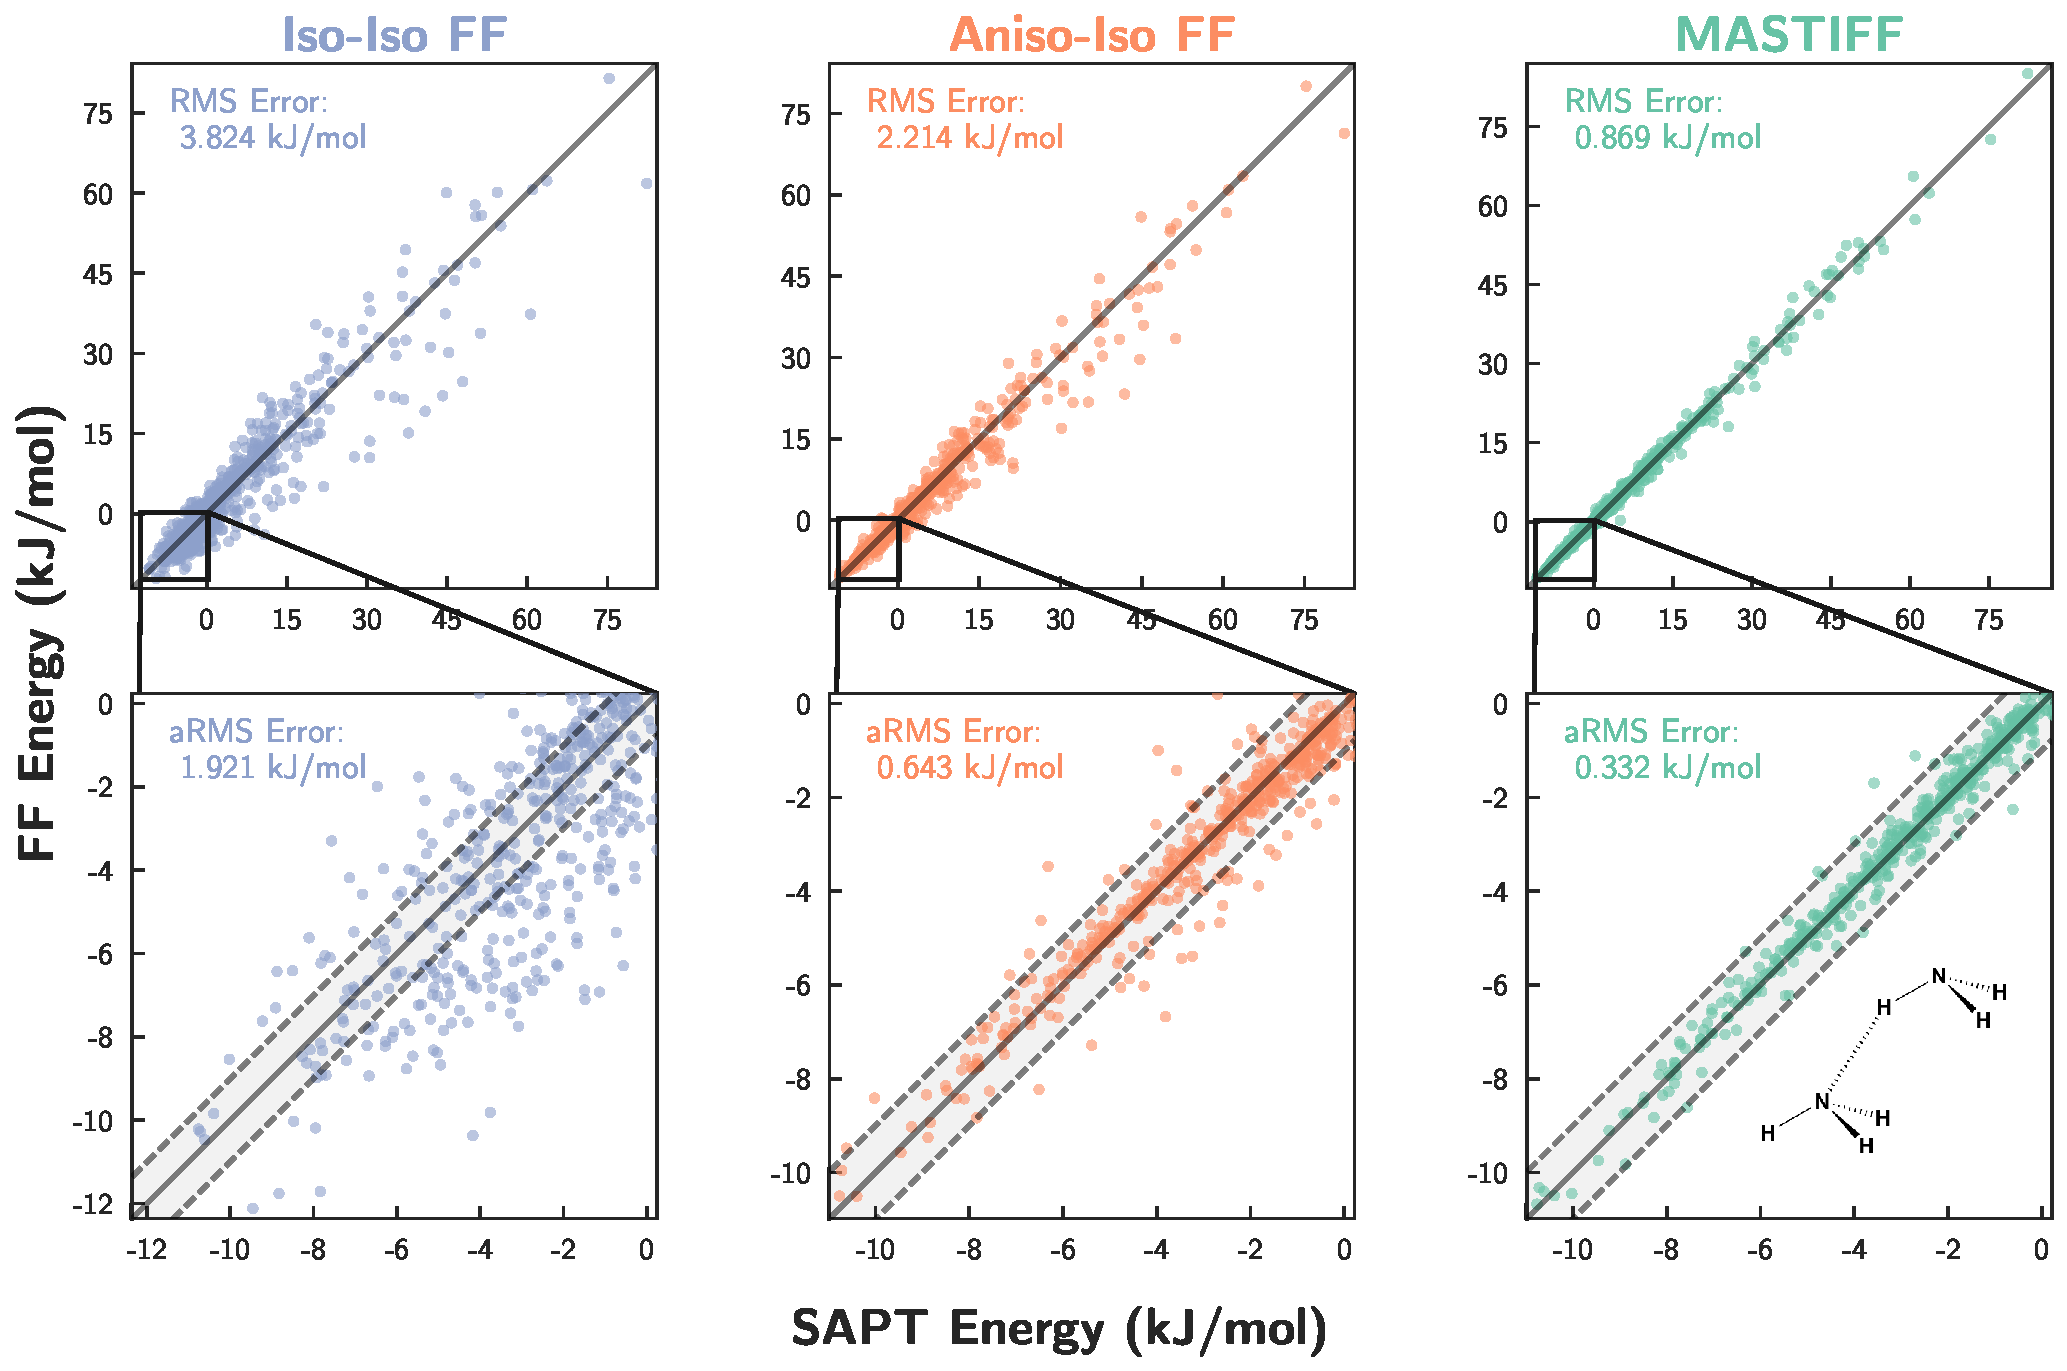
\includegraphics[width=0.9\textwidth]{anisotropic/si/homodimer_figures/nh3_nh3_comparison.pdf}
    \end{subfigure}
    \caption{
    Force field fits for each homomoneric systems using the \isoff (purple),
\isaff (orange), and \mastiff (purple). 
    Two views of the fit to the total energy are displayed along with
    corresponding RMSE (aRMSE for the inset showing attractive configurations). 
    The $y=x$ line (black) indicates perfect agreement between reference energies
    and each force field, while shaded grey areas represent points within $\pm
    1$ kJ/mol agreement of the benchmark. 
     }
    \label{fig:all-scatter}
    \end{figure}
    %%%%%%%% All Scatter %%%%%%%%%%

\end{section}
\clearpage

%\begin{section}{\mastiff-CC energies for \co}
%\begin{section}{2- and 3-body \mastiff-CC \BPChem{CO\_2} energies}
\begin{section}{2- and 3-body \mastiff-CC \texorpdfstring{\co} {} energies}
\label{sec:mastiff-co2_snapshots}

    %%%%%%%%%%%% Average MSE %%%%%%%%%%%%%%%
    \begin{figure}
      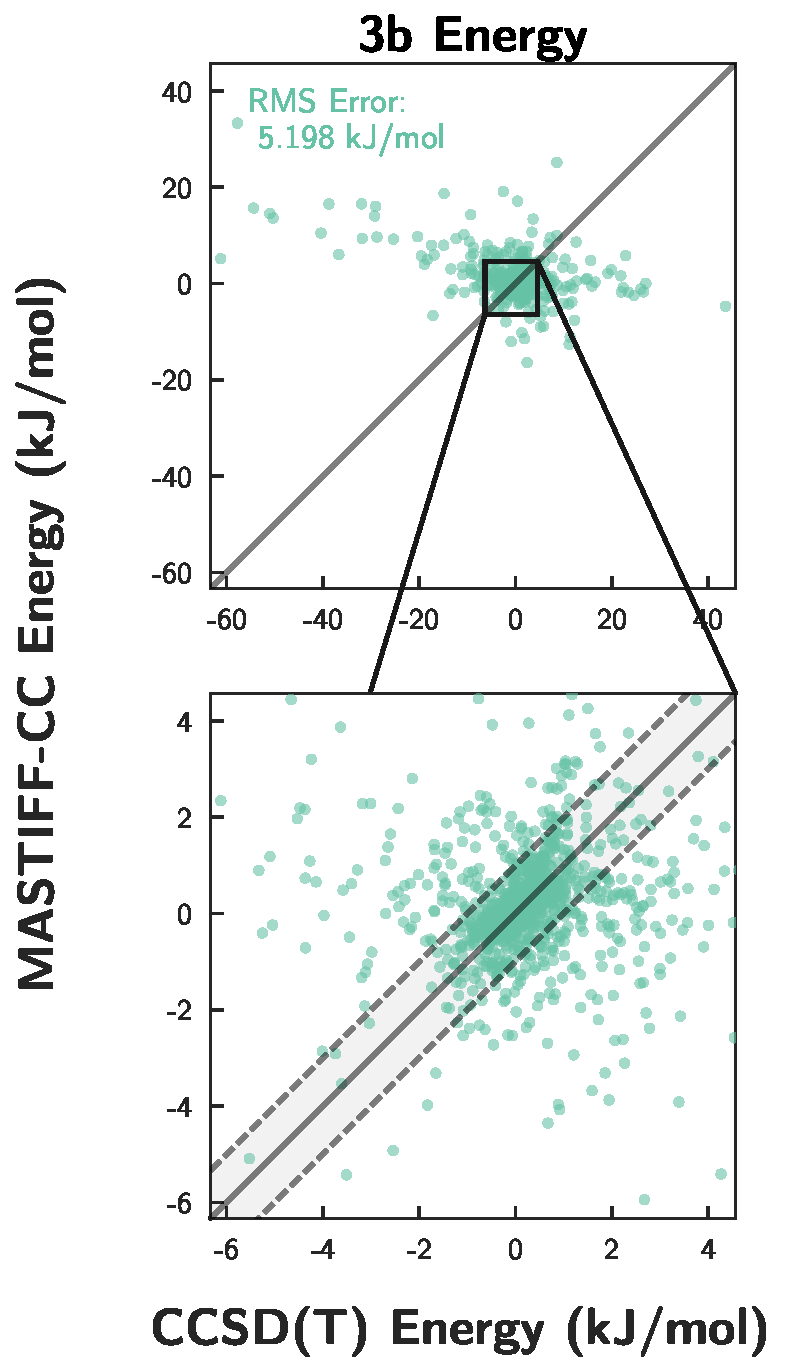
\includegraphics[height=0.8\textwidth]{anisotropic/si/co2_snapshots/trimers_helmann/co2_trimer_comparison.pdf}
        \caption{
        Three-body interaction energies for \co as compared to the
        \citeboth{Hellmann2017} database of
        9401 reference trimer configurations computed at a CCSD(T) level of theory.
                }
    \label{fig:hellmann}
    \end{figure}
    %%%%%%%%%%%% Average MSE %%%%%%%%%%%%%%%

    %%%%%%%%%%%% Average MSE %%%%%%%%%%%%%%%
    \begin{figure}
      \centering
      \begin{minipage}[b]{0.4\textwidth}
      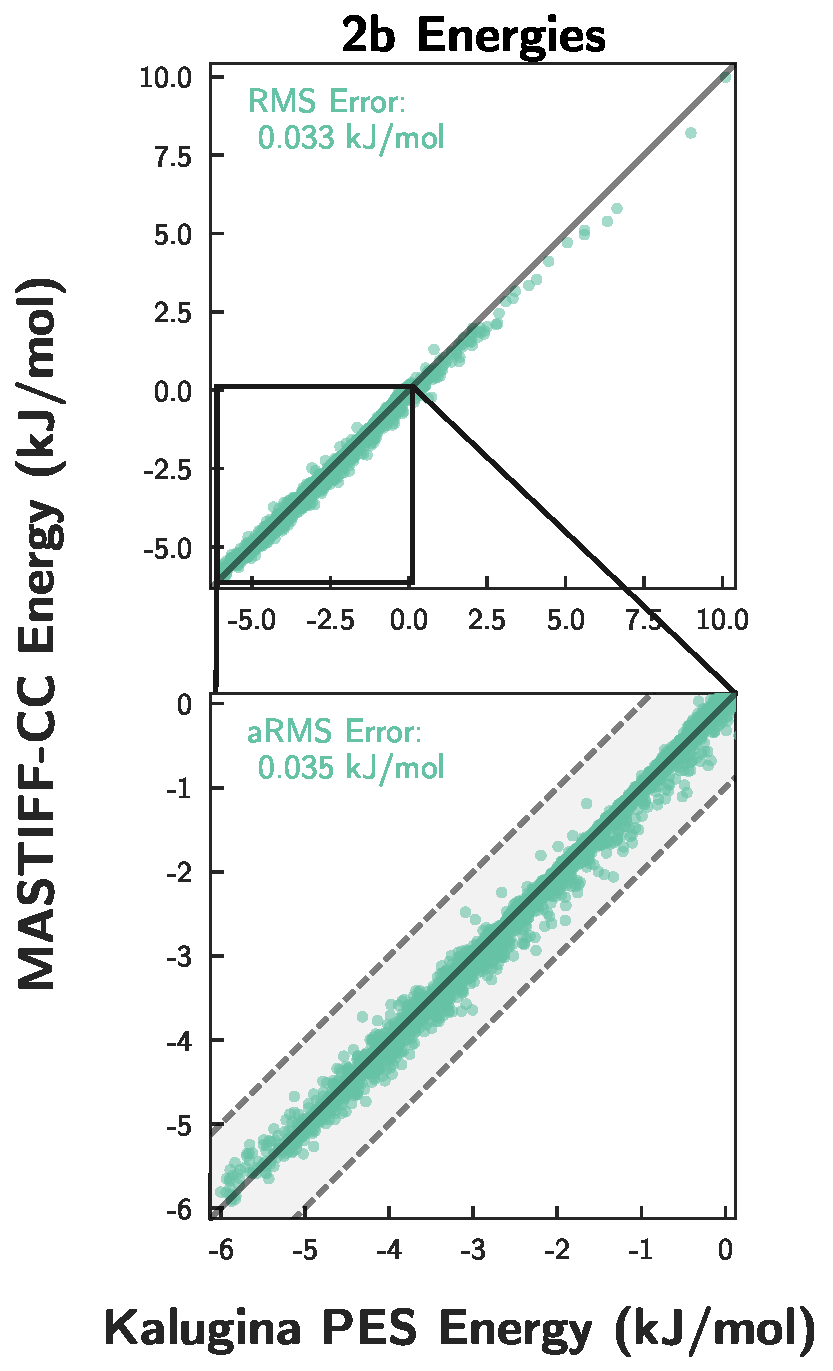
\includegraphics[height=2\textwidth]{anisotropic/si/co2_snapshots/dimer_snapshot/co2_dimer_comparison.pdf}
      \end{minipage}
      \hfill
      \begin{minipage}[b]{0.4\textwidth}
      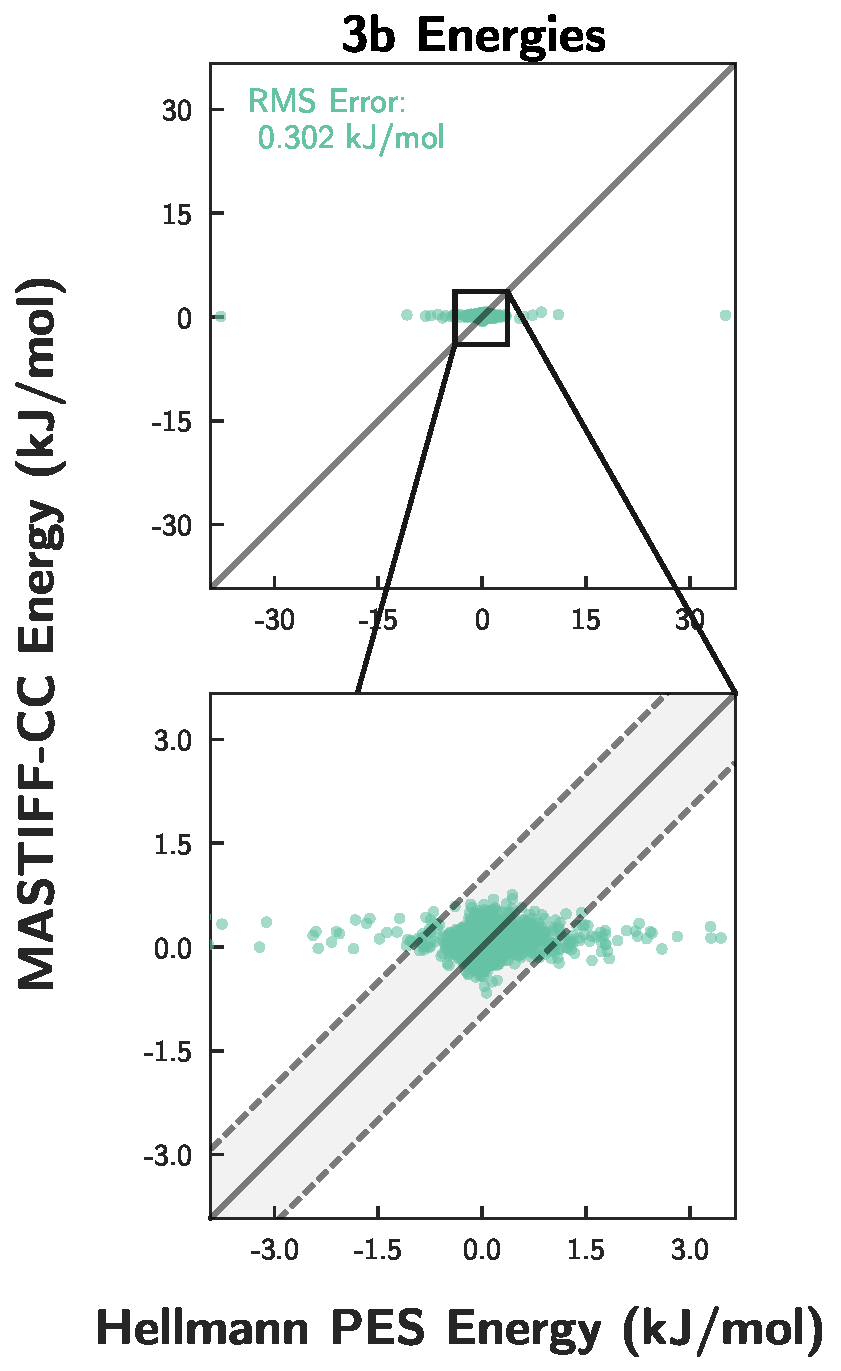
\includegraphics[height=2\textwidth]{anisotropic/si/co2_snapshots/trimers_snapshot/co2_trimer_comparison.pdf}
      \end{minipage}
        \caption{
        Force field quality for \mastiff-CC in reproducing (left) two-body and
(right) three-body \co interaction energies. The $y=x$ line (solid) and $\pm 1$
kJ/mol boundaries (dashed lines) are shown for reference. All dimer/trimer configurations were 
taken from a snapshot of \co liquid simulated using \mastiff-CC at 273.15 K and 100 bar.
Reference energies are taken from the \citeboth{Kalugina2014} PES for the
two-body energies, and the \citeboth{Hellmann2017} PES for the three-body
energies. A total of 62,583 dimer configurations and 43,784 trimer
configurations are represented in the two plots.
                }
    \label{fig:2b_3b_comparison}
    \end{figure}
    %%%%%%%%%%%% Average MSE %%%%%%%%%%%%%%%


\end{section}
%% \clearpage
%% 
%% \singlespacing
%% 
%% \renewcommand{\baselinestretch}{1}
%% 
%% \bibliographystyle{achemso}
%% \bibliography{../library}
%% %\bibliography{rp_extras}
%% 
%% 
%% \end{document}
